% Options for packages loaded elsewhere
\PassOptionsToPackage{unicode}{hyperref}
\PassOptionsToPackage{hyphens}{url}
\PassOptionsToPackage{dvipsnames,svgnames,x11names}{xcolor}
%
\documentclass[
  letterpaper,
  DIV=11,
  numbers=noendperiod]{scrreprt}

\usepackage{amsmath,amssymb}
\usepackage{lmodern}
\usepackage{iftex}
\ifPDFTeX
  \usepackage[T1]{fontenc}
  \usepackage[utf8]{inputenc}
  \usepackage{textcomp} % provide euro and other symbols
\else % if luatex or xetex
  \usepackage{unicode-math}
  \defaultfontfeatures{Scale=MatchLowercase}
  \defaultfontfeatures[\rmfamily]{Ligatures=TeX,Scale=1}
\fi
% Use upquote if available, for straight quotes in verbatim environments
\IfFileExists{upquote.sty}{\usepackage{upquote}}{}
\IfFileExists{microtype.sty}{% use microtype if available
  \usepackage[]{microtype}
  \UseMicrotypeSet[protrusion]{basicmath} % disable protrusion for tt fonts
}{}
\makeatletter
\@ifundefined{KOMAClassName}{% if non-KOMA class
  \IfFileExists{parskip.sty}{%
    \usepackage{parskip}
  }{% else
    \setlength{\parindent}{0pt}
    \setlength{\parskip}{6pt plus 2pt minus 1pt}}
}{% if KOMA class
  \KOMAoptions{parskip=half}}
\makeatother
\usepackage{xcolor}
\setlength{\emergencystretch}{3em} % prevent overfull lines
\setcounter{secnumdepth}{5}
% Make \paragraph and \subparagraph free-standing
\ifx\paragraph\undefined\else
  \let\oldparagraph\paragraph
  \renewcommand{\paragraph}[1]{\oldparagraph{#1}\mbox{}}
\fi
\ifx\subparagraph\undefined\else
  \let\oldsubparagraph\subparagraph
  \renewcommand{\subparagraph}[1]{\oldsubparagraph{#1}\mbox{}}
\fi

\usepackage{color}
\usepackage{fancyvrb}
\newcommand{\VerbBar}{|}
\newcommand{\VERB}{\Verb[commandchars=\\\{\}]}
\DefineVerbatimEnvironment{Highlighting}{Verbatim}{commandchars=\\\{\}}
% Add ',fontsize=\small' for more characters per line
\usepackage{framed}
\definecolor{shadecolor}{RGB}{241,243,245}
\newenvironment{Shaded}{\begin{snugshade}}{\end{snugshade}}
\newcommand{\AlertTok}[1]{\textcolor[rgb]{0.68,0.00,0.00}{#1}}
\newcommand{\AnnotationTok}[1]{\textcolor[rgb]{0.37,0.37,0.37}{#1}}
\newcommand{\AttributeTok}[1]{\textcolor[rgb]{0.40,0.45,0.13}{#1}}
\newcommand{\BaseNTok}[1]{\textcolor[rgb]{0.68,0.00,0.00}{#1}}
\newcommand{\BuiltInTok}[1]{\textcolor[rgb]{0.00,0.23,0.31}{#1}}
\newcommand{\CharTok}[1]{\textcolor[rgb]{0.13,0.47,0.30}{#1}}
\newcommand{\CommentTok}[1]{\textcolor[rgb]{0.37,0.37,0.37}{#1}}
\newcommand{\CommentVarTok}[1]{\textcolor[rgb]{0.37,0.37,0.37}{\textit{#1}}}
\newcommand{\ConstantTok}[1]{\textcolor[rgb]{0.56,0.35,0.01}{#1}}
\newcommand{\ControlFlowTok}[1]{\textcolor[rgb]{0.00,0.23,0.31}{#1}}
\newcommand{\DataTypeTok}[1]{\textcolor[rgb]{0.68,0.00,0.00}{#1}}
\newcommand{\DecValTok}[1]{\textcolor[rgb]{0.68,0.00,0.00}{#1}}
\newcommand{\DocumentationTok}[1]{\textcolor[rgb]{0.37,0.37,0.37}{\textit{#1}}}
\newcommand{\ErrorTok}[1]{\textcolor[rgb]{0.68,0.00,0.00}{#1}}
\newcommand{\ExtensionTok}[1]{\textcolor[rgb]{0.00,0.23,0.31}{#1}}
\newcommand{\FloatTok}[1]{\textcolor[rgb]{0.68,0.00,0.00}{#1}}
\newcommand{\FunctionTok}[1]{\textcolor[rgb]{0.28,0.35,0.67}{#1}}
\newcommand{\ImportTok}[1]{\textcolor[rgb]{0.00,0.46,0.62}{#1}}
\newcommand{\InformationTok}[1]{\textcolor[rgb]{0.37,0.37,0.37}{#1}}
\newcommand{\KeywordTok}[1]{\textcolor[rgb]{0.00,0.23,0.31}{#1}}
\newcommand{\NormalTok}[1]{\textcolor[rgb]{0.00,0.23,0.31}{#1}}
\newcommand{\OperatorTok}[1]{\textcolor[rgb]{0.37,0.37,0.37}{#1}}
\newcommand{\OtherTok}[1]{\textcolor[rgb]{0.00,0.23,0.31}{#1}}
\newcommand{\PreprocessorTok}[1]{\textcolor[rgb]{0.68,0.00,0.00}{#1}}
\newcommand{\RegionMarkerTok}[1]{\textcolor[rgb]{0.00,0.23,0.31}{#1}}
\newcommand{\SpecialCharTok}[1]{\textcolor[rgb]{0.37,0.37,0.37}{#1}}
\newcommand{\SpecialStringTok}[1]{\textcolor[rgb]{0.13,0.47,0.30}{#1}}
\newcommand{\StringTok}[1]{\textcolor[rgb]{0.13,0.47,0.30}{#1}}
\newcommand{\VariableTok}[1]{\textcolor[rgb]{0.07,0.07,0.07}{#1}}
\newcommand{\VerbatimStringTok}[1]{\textcolor[rgb]{0.13,0.47,0.30}{#1}}
\newcommand{\WarningTok}[1]{\textcolor[rgb]{0.37,0.37,0.37}{\textit{#1}}}

\providecommand{\tightlist}{%
  \setlength{\itemsep}{0pt}\setlength{\parskip}{0pt}}\usepackage{longtable,booktabs,array}
\usepackage{calc} % for calculating minipage widths
% Correct order of tables after \paragraph or \subparagraph
\usepackage{etoolbox}
\makeatletter
\patchcmd\longtable{\par}{\if@noskipsec\mbox{}\fi\par}{}{}
\makeatother
% Allow footnotes in longtable head/foot
\IfFileExists{footnotehyper.sty}{\usepackage{footnotehyper}}{\usepackage{footnote}}
\makesavenoteenv{longtable}
\usepackage{graphicx}
\makeatletter
\def\maxwidth{\ifdim\Gin@nat@width>\linewidth\linewidth\else\Gin@nat@width\fi}
\def\maxheight{\ifdim\Gin@nat@height>\textheight\textheight\else\Gin@nat@height\fi}
\makeatother
% Scale images if necessary, so that they will not overflow the page
% margins by default, and it is still possible to overwrite the defaults
% using explicit options in \includegraphics[width, height, ...]{}
\setkeys{Gin}{width=\maxwidth,height=\maxheight,keepaspectratio}
% Set default figure placement to htbp
\makeatletter
\def\fps@figure{htbp}
\makeatother
\newlength{\cslhangindent}
\setlength{\cslhangindent}{1.5em}
\newlength{\csllabelwidth}
\setlength{\csllabelwidth}{3em}
\newlength{\cslentryspacingunit} % times entry-spacing
\setlength{\cslentryspacingunit}{\parskip}
\newenvironment{CSLReferences}[2] % #1 hanging-ident, #2 entry spacing
 {% don't indent paragraphs
  \setlength{\parindent}{0pt}
  % turn on hanging indent if param 1 is 1
  \ifodd #1
  \let\oldpar\par
  \def\par{\hangindent=\cslhangindent\oldpar}
  \fi
  % set entry spacing
  \setlength{\parskip}{#2\cslentryspacingunit}
 }%
 {}
\usepackage{calc}
\newcommand{\CSLBlock}[1]{#1\hfill\break}
\newcommand{\CSLLeftMargin}[1]{\parbox[t]{\csllabelwidth}{#1}}
\newcommand{\CSLRightInline}[1]{\parbox[t]{\linewidth - \csllabelwidth}{#1}\break}
\newcommand{\CSLIndent}[1]{\hspace{\cslhangindent}#1}

\KOMAoption{captions}{tableheading}
\makeatletter
\makeatother
\makeatletter
\@ifpackageloaded{bookmark}{}{\usepackage{bookmark}}
\makeatother
\makeatletter
\@ifpackageloaded{caption}{}{\usepackage{caption}}
\AtBeginDocument{%
\ifdefined\contentsname
  \renewcommand*\contentsname{Table of contents}
\else
  \newcommand\contentsname{Table of contents}
\fi
\ifdefined\listfigurename
  \renewcommand*\listfigurename{List of Figures}
\else
  \newcommand\listfigurename{List of Figures}
\fi
\ifdefined\listtablename
  \renewcommand*\listtablename{List of Tables}
\else
  \newcommand\listtablename{List of Tables}
\fi
\ifdefined\figurename
  \renewcommand*\figurename{Figure}
\else
  \newcommand\figurename{Figure}
\fi
\ifdefined\tablename
  \renewcommand*\tablename{Table}
\else
  \newcommand\tablename{Table}
\fi
}
\@ifpackageloaded{float}{}{\usepackage{float}}
\floatstyle{ruled}
\@ifundefined{c@chapter}{\newfloat{codelisting}{h}{lop}}{\newfloat{codelisting}{h}{lop}[chapter]}
\floatname{codelisting}{Listing}
\newcommand*\listoflistings{\listof{codelisting}{List of Listings}}
\makeatother
\makeatletter
\@ifpackageloaded{caption}{}{\usepackage{caption}}
\@ifpackageloaded{subcaption}{}{\usepackage{subcaption}}
\makeatother
\makeatletter
\@ifpackageloaded{tcolorbox}{}{\usepackage[many]{tcolorbox}}
\makeatother
\makeatletter
\@ifundefined{shadecolor}{\definecolor{shadecolor}{rgb}{.97, .97, .97}}
\makeatother
\makeatletter
\makeatother
\ifLuaTeX
  \usepackage{selnolig}  % disable illegal ligatures
\fi
\IfFileExists{bookmark.sty}{\usepackage{bookmark}}{\usepackage{hyperref}}
\IfFileExists{xurl.sty}{\usepackage{xurl}}{} % add URL line breaks if available
\urlstyle{same} % disable monospaced font for URLs
\hypersetup{
  pdftitle={Deep Learning with TensorFlow 2},
  colorlinks=true,
  linkcolor={blue},
  filecolor={Maroon},
  citecolor={Blue},
  urlcolor={Blue},
  pdfcreator={LaTeX via pandoc}}

\title{Deep Learning with TensorFlow 2}
\author{}
\date{}

\begin{document}
\maketitle
\ifdefined\Shaded\renewenvironment{Shaded}{\begin{tcolorbox}[boxrule=0pt, sharp corners, enhanced, breakable, borderline west={3pt}{0pt}{shadecolor}, frame hidden, interior hidden]}{\end{tcolorbox}}\fi

\renewcommand*\contentsname{Table of contents}
{
\hypersetup{linkcolor=}
\setcounter{tocdepth}{2}
\tableofcontents
}
\bookmarksetup{startatroot}

\hypertarget{welcome}{%
\chapter*{Welcome}\label{welcome}}
\addcontentsline{toc}{chapter}{Welcome}

\markboth{Welcome}{Welcome}

Welcome to for \textbf{Deep Learning using TensorFlow 2}, a book that
will show you how to use TensorFlow 2 to build and train your own
models. In this book, you will learn how to use TensorFlow 2 and its
high-level API, Keras, to implement various deep learning techniques,
such as artificial neural networks, convolutional neural networks,
recurrent neural networks, and more. In addition, several approaches to
deal with different types of data, such as image, text, and time series
data, will be discussed. You will learn the fundamental of TensorFlow 2
for use cases in some of the most popular and challenging domains of
deep learning, which are computer vision, natural language processing,
and time series data.

This book is designed for beginners who want to learn TensorFlow 2 from
scratch by practicing the techniques on practical examples and projects.
Whether you are new to TensorFlow or have some experience with it, this
book will help you master the essential skills and concepts you need to
create effective solutions for real-world problems. Nevertheless, you
are assumed to have some backgrounds in Python programming. Each chapter
provides a brief introduction to the theory behind each technique,
followed by a step-by-step guide on how to implement it using TensorFlow
2, Keras, and other relevant libraries.

By the end of this book, you will have a solid foundation in TensorFlow
2 and deep learning, and you will be able to use your skills and
knowledge to create your own projects or advance your career in this
exciting and fast-growing field.

\hypertarget{collaboration}{%
\subsection*{Collaboration}\label{collaboration}}
\addcontentsline{toc}{subsection}{Collaboration}

This book is \textbf{currently under development}. The 1source code for
this website is available on
\href{https://github.com/hanzholahs/tensorflow-for-deep-learning}{GitHub}.
We welcome any contributions or feedback from other developers who are
interested in this project. If you find any errors or typos, please feel
free to open an issue or a pull request. Thank you for your support and
collaboration.

\hypertarget{authors}{%
\subsection*{Authors}\label{authors}}
\addcontentsline{toc}{subsection}{Authors}

\begin{enumerate}
\def\labelenumi{\arabic{enumi}.}
\item
  \textbf{Hanzholah Shobri}, a Researcher at Bank Indonesia. He hold a
  bachelor's degree in Industrial Engineering from Universitas Gadjah
  Mada, Yogyakarta. (contacts:
  \href{mailto:hanzholahs@gmail.com}{email},
  \href{https://github.com/hanzholahs}{github},
  \href{https://twitter.com/hanzholah}{twitter})
\item
  \textbf{Tria Rahmat Mauludin}, a Researcher at Bank Indonesia. He hold
  a bachelor's degree in Mathematics from Insitut Teknologi Bandung,
  Bandung. (contacts: \href{mailto:triarahmatm@gmail.com}{email},
  \href{https://github.com/triarm}{github})
\end{enumerate}

\hypertarget{license}{%
\subsection*{License}\label{license}}
\addcontentsline{toc}{subsection}{License}

This book is licensed to you under
\href{https://creativecommons.org/licenses/by-nc-nd/4.0/}{Creative
Commons Attribution-NonCommercial-NoDerivatives 4.0 International
License}.

The code samples in this book are licensed under
\href{https://creativecommons.org/publicdomain/zero/1.0/}{Creative
Commons CC0 1.0 Universal (CC0 1.0)}, i.e.~public domain.

\bookmarksetup{startatroot}

\hypertarget{introduction}{%
\chapter*{Introduction}\label{introduction}}
\addcontentsline{toc}{chapter}{Introduction}

\markboth{Introduction}{Introduction}

Deep learning is a branch of artificial intelligence that uses neural
networks to learn from data and perform certain tasks. Many creative and
innnovative solutions to human problems have been solved by deep
learning techniques. Hence, the skills to use deep learning in any
domain is important in the era where computational capabilty and data
availability is continally increasing. This book consists of the
application of several key techniques in deep learning to deal with
complex data structures.

If you are familiar with Python and want to learn TensorFlow by solving
real-world problems, this book is for you. You will learn how to use
TensorFlow to build machine learning models for various domains, such as
computer vision, natural language processing, and more. You will also
get hands-on experience with TensorFlow through case studies and
practical examples that show you how to apply the concepts and
techniques in your own projects. Every relevant concept is introduced
gradually, so it is recommended to read the book from the first chapter
to the end.

\hypertarget{the-concepts-of-artificial-intelligence-machine-learning-and-deep-learning}{%
\subsection*{The concepts of Artificial Intelligence, Machine Learning,
and Deep
Learning}\label{the-concepts-of-artificial-intelligence-machine-learning-and-deep-learning}}
\addcontentsline{toc}{subsection}{The concepts of Artificial
Intelligence, Machine Learning, and Deep Learning}

To understand what deep learning is, we need to also look at the
definition of machine learning and deep learning. In principle, deep
learning is a subset of machine learning, and machine learning is a
subset of artificial intelligence.

Artificial intelligence (AI) is a broad term that refers to any system
or software that can perform tasks that normally require human
intelligence, such as reasoning, decision making, problem solving,
natural language processing, and computer vision. Machine learning (ML)
is a subset of AI that focuses on creating systems or software that can
learn patterns or rules from data and improve their performance without
explicit programming or human intervention.

Deep learning (DL) is a subset of ML that uses artificial neural
networks (ANNs) to model complex and nonlinear relationships between
inputs and outputs. In contrast to traditional machine learning that
requires manual feature engineering to extract relevant information,
deep learning uses multiple intermediate representations of the data to
extract features automatically from raw data.

An illustration by Data Iku on the relationship between AI, ML, and DL
is presented below.

\begin{figure}

{\centering \includegraphics{https://blog.dataiku.com/hs-fs/hubfs/AI-ML-DL-graphic.png?width=810\&name=AI-ML-DL-graphic.png}

}

\caption{DL is a subset of ML, and ML is a subset of AI}

\end{figure}

\hypertarget{an-introduction-to-tensorflow-2.0-and-keras-libraries}{%
\subsection*{An Introduction to TensorFlow 2.0 and Keras
Libraries}\label{an-introduction-to-tensorflow-2.0-and-keras-libraries}}
\addcontentsline{toc}{subsection}{An Introduction to TensorFlow 2.0 and
Keras Libraries}

Tensorflow 2 and Keras are two powerful frameworks for building and
deploying machine learning solutions, especially for deep learning.
Tensorflow 2 is the premier open-source platform for developing,
training, and deploying deep learning models at scale. Keras is the
high-level API of Tensorflow 2, which provides an easy and intuitive way
to design, fit, evaluate, and use deep learning models with just a few
lines of code.

Tensorflow 2 and Keras have many advantages over other frameworks, such
as:

\begin{itemize}
\tightlist
\item
  They support multiple backends, devices, and languages, allowing you
  to run your code on CPUs, GPUs, TPUs, and even mobile devices.
\item
  They offer a rich set of tools and libraries for data processing,
  visualization, debugging, optimization, and deployment.
\item
  They enable you to use both the sequential and functional APIs to
  create simple or complex models with different architectures and
  layers.
\item
  They allow you to leverage the power of custom layers, custom training
  loops, custom callbacks, and custom metrics to customize your model
  according to your needs.
\item
  They integrate seamlessly with other popular libraries and frameworks,
  such as NumPy, SciPy, Pandas, Scikit-learn, PyTorch, and more.
\end{itemize}

Tensorflow 2 and Keras are not only frameworks but also communities of
developers, researchers, and practitioners who share their knowledge and
experience through blogs, tutorials, books, courses, forums, and events.
By using Tensorflow 2 and Keras, you can join this vibrant community and
learn from the best in the field.

\hypertarget{how-will-you-learn-deep-learning-by-using-this-book}{%
\subsection*{How Will You Learn Deep Learning by Using This
Book?}\label{how-will-you-learn-deep-learning-by-using-this-book}}
\addcontentsline{toc}{subsection}{How Will You Learn Deep Learning by
Using This Book?}

This book exclusively uses TensorFlow 2, as well as its high-level API
or Keras, to build and train a deep learning model. Other libraries are
also used for preparing the data or making visualisation. To practice
with the code in this book, readers could access the source notebook or
copy and paste each code manually. There are three parts of the book.

\begin{itemize}
\tightlist
\item
  \textbf{Part 1: Basic Usage of TensorFlow 2}. This part contains the
  basic workflow to build a model that is used in this book and how to
  implement TensorFlow 2 according to the workflow for regression and
  classification problems using dummy data.
\item
  \textbf{Part 2: Use Cases of TensorFlow 2}. This part demonstrates
  several applications of some important techniques in machine learning
  and TensorFlow 2 to four use cases using datasets provided by
  TensorFlow 2 library.
\item
  \textbf{Part 3: Preparing Data for TensorFlow 2}. This part goes
  beyond built-in dataset and shows how to handle messy, real-world data
  in different formats (images, texts, and time series data) into inputs
  for TensorFlow 2 deep learning models.
\end{itemize}

\part{{Basic Usage of TensorFlow 2}}

\hypertarget{general-workflow-for-this-book}{%
\chapter{General Workflow for This
Book}\label{general-workflow-for-this-book}}

Deep learning is a powerful and popular branch of machine learning that
uses neural networks to learn from data and perform complex tasks. In
this blog post, we will explore the typical workflow of a deep learning
project, and discuss some of the relevant libraries, tools and
techniques that can help you along the way.

The deep learning workflow has seven primary components:

\begin{enumerate}
\def\labelenumi{\arabic{enumi}.}
\tightlist
\item
  \textbf{Acquiring data}: This is the first and often the most
  challenging step of a deep learning project. You need to collect
  enough labeled data for your task, or use existing datasets that are
  publicly available or stored in databases. You can also use web
  scraping or APIs to gather data from online sources, or crowd-source
  labeling for unlabeled data.
\item
  \textbf{Preprocessing}: This step involves cleaning, transforming and
  organizing your data to make it suitable for your model. You may need
  to resize, crop, rotate, augment or normalize your images; tokenize,
  lemmatize, stem or vectorize your text; encode, scale, impute or
  standardize your numerical data; and so on. You can use libraries like
  NumPy, Pandas, OpenCV, PIL, NLTK or Scikit-learn for preprocessing
  tasks.
\item
  \textbf{Splitting and balancing the dataset}: This step involves
  dividing your data into training, validation and test sets. The
  training set is used to fit the model to the data; the validation set
  is used to tune the hyperparameters and select the best model; and the
  test set is used to evaluate the final performance of the model. You
  should also ensure that your dataset is balanced, meaning that it has
  roughly equal proportions of different classes or categories. You can
  use Scikit-learn's train\_test\_split function or TensorFlow's tf.data
  API for splitting and balancing your dataset.
\item
  \textbf{Defining model architecture}: This step involves designing the
  structure and layers of your neural network. You can use existing
  architectures that have been proven to work well for similar tasks,
  such as CNNs for image classification, RNNs for natural language
  processing, GANs for image generation, etc. You can also modify or
  customize these architectures to suit your specific needs. You can use
  libraries like TensorFlow, Keras, PyTorch or MXNet for defining your
  model architecture.
\item
  \textbf{Fitting model to data}: This step involves training your model
  on the training set using an optimization algorithm such as gradient
  descent. You need to specify the loss function that measures how well
  your model fits the data, and the metrics that evaluate how well your
  model performs on the validation set. You also need to choose the
  learning rate, batch size, number of epochs and other hyperparameters
  that affect the speed and quality of training. You can use libraries
  like TensorFlow, Keras, PyTorch or MXNet for fitting your model to
  data.
\item
  \textbf{Making predictions}: This step involves using your trained
  model to make predictions on new or unseen data. You can use your
  model to classify images, generate text, translate languages, detect
  objects, etc. depending on your task. You can use libraries like
  TensorFlow, Keras, PyTorch or MXNet for making predictions.
\item
  \textbf{Evaluating results}: This step involves measuring how well
  your model performs on the test set using various metrics such as
  accuracy, precision, recall, F1-score, ROC curve, etc. depending on
  your task. You can also compare your results with existing benchmarks
  or state-of-the-art models to see how you fare against them. You can
  use libraries like Scikit-learn, TensorFlow or PyTorch for evaluating
  results.
\item
  \textbf{Model optimization}: This step involves improving your model
  by fine-tuning the hyperparameters, adding regularization techniques
  such as dropout or batch normalization, pruning unnecessary weights or
  layers, etc. You can also use techniques such as transfer learning or
  meta-learning to leverage existing knowledge or learn from multiple
  tasks. You can use libraries like TensorFlow Hub or PyTorch Lightning
  for model optimization.
\end{enumerate}

As you can see, deep learning workflow is an iterative and dynamic
process that requires a lot of experimentation and creativity. However,
by following these steps and using these libraries and tools, you can
make your deep learning project more productive, reproducible and
understandable.

\hypertarget{dealing-with-regression-problems}{%
\chapter{Dealing with Regression
Problems}\label{dealing-with-regression-problems}}

TensorFlow 2 (TF2) provides a whole set of tools to implement machine
learning to a wide range of problems, from preparing the data to
deploying a model. In this post, I demonstrate how to use the package to
build a regression model predicting continuous numerical values based on
input data.

The objective of this demo is to show you the main elements of working
with a TF2 model to tackle regression problems.

Important libraries are loaded, namely \texttt{tensorflow},
\texttt{numpy} to manipulate data, \texttt{pandas} to deal with table,
and \texttt{seaborn} to create visualisation. As part of the setup, I
also clean the \texttt{TF2} environment with \texttt{clear\_session}
function and set seed for random number generation using
\texttt{set\_random\_seed} function.

For the visualisation, I attempted to use the \texttt{seaborn.objects}
interface. The reason for this is that I am familiar with the
\texttt{ggplot2} package in \texttt{R} when conducting data analysis,
and I found that there is some similarity in both approach of creating a
plot. For those who aren't familiar with \texttt{ggplot2} package, it
employs the concept of
\href{https://vita.had.co.nz/papers/layered-grammar.html}{layered
grammar of graphics} allowing you to describe any plots in a more
structured way which result in more convenient and consistent code. You
can see the documentations for the \texttt{seaborn.objects} interface
\href{https://seaborn.pydata.org/tutorial/objects_interface}{here} and
the \texttt{ggplot2} package
\href{https://ggplot2.tidyverse.org/}{here}.

\begin{Shaded}
\begin{Highlighting}[]
\ImportTok{import}\NormalTok{ tensorflow }\ImportTok{as}\NormalTok{ tf}
\ImportTok{import}\NormalTok{ numpy }\ImportTok{as}\NormalTok{ np}
\ImportTok{import}\NormalTok{ pandas }\ImportTok{as}\NormalTok{ pd}
\ImportTok{import}\NormalTok{ seaborn.objects }\ImportTok{as}\NormalTok{ so}
\end{Highlighting}
\end{Shaded}

\begin{Shaded}
\begin{Highlighting}[]
\NormalTok{tf.keras.backend.clear\_session()}
\NormalTok{tf.keras.utils.set\_random\_seed(}\DecValTok{123}\NormalTok{)}
\end{Highlighting}
\end{Shaded}

\hypertarget{generate-random-data}{%
\section{Generate Random Data}\label{generate-random-data}}

For the sample problem, I generated a 1000 observations of random number
with two independent variables \(x_0\) and \(x_1\). The target for
prediction is calculated using simple formula below.

\[
    y = f(x) = 0.2 \times x_0 + 2.8 \times x_1 + \epsilon 
\]

All variables \(x_0\) and \(x_1\) as well as the error term \(\epsilon\)
follow a normal distribution \(N(\mu, \sigma^2)\) with \(\mu = 0\) and
\(\sigma^2 = 1\).

\begin{Shaded}
\begin{Highlighting}[]
\NormalTok{X }\OperatorTok{=}\NormalTok{ np.random.normal(size }\OperatorTok{=}\NormalTok{ (}\DecValTok{1000}\NormalTok{, }\DecValTok{2}\NormalTok{))}
\NormalTok{y }\OperatorTok{=} \FloatTok{0.2} \OperatorTok{*}\NormalTok{ X[:, }\DecValTok{0}\NormalTok{] }\OperatorTok{+} \FloatTok{2.8} \OperatorTok{*}\NormalTok{ X[:, }\DecValTok{1}\NormalTok{] }\OperatorTok{+}\NormalTok{ np.random.normal(size }\OperatorTok{=}\NormalTok{ (}\DecValTok{1000}\NormalTok{,))}
\end{Highlighting}
\end{Shaded}

For evaluation of model, I split the data, 80\% for training and 20\%
for testing.

\begin{Shaded}
\begin{Highlighting}[]
\NormalTok{X\_train }\OperatorTok{=}\NormalTok{ X[:}\DecValTok{800}\NormalTok{]}
\NormalTok{y\_train }\OperatorTok{=}\NormalTok{ y[:}\DecValTok{800}\NormalTok{]}
\NormalTok{X\_test }\OperatorTok{=}\NormalTok{ X[}\DecValTok{800}\NormalTok{:]}
\NormalTok{y\_test }\OperatorTok{=}\NormalTok{ y[}\DecValTok{800}\NormalTok{:]}

\NormalTok{X\_train.shape, y\_train.shape, X\_test.shape, y\_test.shape, }
\end{Highlighting}
\end{Shaded}

\begin{verbatim}
((800, 2), (800,), (200, 2), (200,))
\end{verbatim}

\hypertarget{a-very-simple-tf2-model}{%
\section{\texorpdfstring{A Very Simple \texttt{TF2}
Model}{A Very Simple TF2 Model}}\label{a-very-simple-tf2-model}}

\hypertarget{defining-the-model}{%
\subsection{Defining the model}\label{defining-the-model}}

Defining a \texttt{TF2} model can be accomplished easily by calling the
\texttt{Sequential} method, followed by \texttt{add}ing any types and
number of layers. As the problem is very straightforward, tackling this
should be relatively easy. For this reason, the model I defined here is
very simple with only one \texttt{Dense} layer with one perceptron unit.
In addition, we need to define the \texttt{input\_shape} so that the
model can determine the number of parameters it requires to predict all
inputs. The \texttt{summary} method allows you to see the architecture
of the model.

\begin{Shaded}
\begin{Highlighting}[]
\NormalTok{model }\OperatorTok{=}\NormalTok{ tf.keras.models.Sequential()}
\NormalTok{model.add(tf.keras.layers.Dense(}\DecValTok{1}\NormalTok{, input\_shape }\OperatorTok{=}\NormalTok{ (}\DecValTok{2}\NormalTok{, )))}
\NormalTok{model.summary()}
\end{Highlighting}
\end{Shaded}

\begin{verbatim}
Model: "sequential"
_________________________________________________________________
 Layer (type)                Output Shape              Param #   
=================================================================
 dense (Dense)               (None, 1)                 3         
                                                                 
=================================================================
Total params: 3
Trainable params: 3
Non-trainable params: 0
_________________________________________________________________
\end{verbatim}

Before training the model, you are required to choose the optimizer,
loss function, and metrics, and \texttt{compile} those into the model.
Here, I decided to use Stochastic Gradient Descent algorithm for
optimizing the model (i.e., updating neural network parameters), Mean
Squared Error (MSE) for determining how far the prediciton of the
current model with actual values, and Mean Absolute Error (MAE) as a
metric to evaluate the model.

\begin{Shaded}
\begin{Highlighting}[]
\NormalTok{model.}\BuiltInTok{compile}\NormalTok{(optimizer }\OperatorTok{=} \StringTok{"sgd"}\NormalTok{, loss }\OperatorTok{=} \StringTok{"mse"}\NormalTok{, metrics }\OperatorTok{=}\NormalTok{ [}\StringTok{"mae"}\NormalTok{])}
\end{Highlighting}
\end{Shaded}

\hypertarget{training-the-model}{%
\subsection{Training the model}\label{training-the-model}}

Training can be done using \texttt{fit} method. The process is done
after 100 \texttt{epochs} or cycles of the model updating its parameters
based on input data. The \texttt{verbose} parameter that equals 0 means
that the training will not print any information.

\begin{Shaded}
\begin{Highlighting}[]
\NormalTok{history }\OperatorTok{=}\NormalTok{ model.fit(X\_train, y\_train, epochs }\OperatorTok{=} \DecValTok{100}\NormalTok{, verbose }\OperatorTok{=} \DecValTok{0}\NormalTok{)}
\end{Highlighting}
\end{Shaded}

The \texttt{fit} method returns \texttt{History} object, which provides
you the performance of the model during training. The
\texttt{history.history} contains all loss and metric scores for all
training epochs, and you can extract this information to evalate your
model. I performed some manipulation basically to have a certain format
of data (the long version, you might want to refer to \href{}{tidy data
by Hadley Wickham}).

\begin{Shaded}
\begin{Highlighting}[]
\NormalTok{data }\OperatorTok{=}\NormalTok{ pd.DataFrame(history.history)}
\NormalTok{data }\OperatorTok{=}\NormalTok{ data.reset\_index()}
\NormalTok{data }\OperatorTok{=}\NormalTok{ data.rename(columns }\OperatorTok{=}\NormalTok{ \{}
    \StringTok{"index"}\NormalTok{:}\StringTok{"epoch"}\NormalTok{, }
    \StringTok{"loss"}\NormalTok{: }\StringTok{"Mean Squared Error"}\NormalTok{, }
    \StringTok{"mae"}\NormalTok{: }\StringTok{"Mean Absolute Error"}\NormalTok{\})}
\NormalTok{data }\OperatorTok{=}\NormalTok{ pd.melt(}
\NormalTok{    data, }
\NormalTok{    id\_vars }\OperatorTok{=} \StringTok{"epoch"}\NormalTok{, }
\NormalTok{    value\_vars }\OperatorTok{=}\NormalTok{ [}\StringTok{"Mean Squared Error"}\NormalTok{, }\StringTok{"Mean Absolute Error"}\NormalTok{],}
\NormalTok{    var\_name }\OperatorTok{=} \StringTok{"metric"}\NormalTok{,}
\NormalTok{    value\_name }\OperatorTok{=} \StringTok{"value"}
\NormalTok{)}

\NormalTok{data.sort\_values(by }\OperatorTok{=} \StringTok{"epoch"}\NormalTok{).head()}
\end{Highlighting}
\end{Shaded}

\begin{longtable}[]{@{}llll@{}}
\toprule()
& epoch & metric & value \\
\midrule()
\endhead
0 & 0 & Mean Squared Error & 5.752564 \\
100 & 0 & Mean Absolute Error & 1.881032 \\
1 & 1 & Mean Squared Error & 2.836762 \\
101 & 1 & Mean Absolute Error & 1.315763 \\
2 & 2 & Mean Squared Error & 1.707698 \\
\bottomrule()
\end{longtable}

We can then visualise how the model perform throughout the training.

\begin{Shaded}
\begin{Highlighting}[]
\NormalTok{(}
\NormalTok{    so.Plot(data, x }\OperatorTok{=} \StringTok{"epoch"}\NormalTok{, y }\OperatorTok{=} \StringTok{"value"}\NormalTok{)}
\NormalTok{    .facet(}\StringTok{"metric"}\NormalTok{)}
\NormalTok{    .add(so.Line())}
\NormalTok{    .share(y }\OperatorTok{=} \VariableTok{False}\NormalTok{)}
\NormalTok{    .limit(y }\OperatorTok{=}\NormalTok{ (}\DecValTok{0}\NormalTok{, }\VariableTok{None}\NormalTok{))}
\NormalTok{    .layout(size }\OperatorTok{=}\NormalTok{ (}\DecValTok{8}\NormalTok{, }\DecValTok{3}\NormalTok{))}
\NormalTok{    .label(x }\OperatorTok{=} \StringTok{""}\NormalTok{, y }\OperatorTok{=} \StringTok{""}\NormalTok{)}
\NormalTok{)}
\end{Highlighting}
\end{Shaded}

\begin{figure}[H]

{\centering \includegraphics{notebooks/01b-basic-regression_files/figure-pdf/cell-10-output-1.png}

}

\end{figure}

\hypertarget{evaluating-the-model}{%
\subsection{Evaluating the model}\label{evaluating-the-model}}

Finally, we can check the model's performance on the test dataset. The
\texttt{evaluate} method allows the users to see how the model perform
when predicting unseen data. The model seems to do good in predicting
the actual output based on the MSE and MAE.

\begin{Shaded}
\begin{Highlighting}[]
\NormalTok{mse, mae }\OperatorTok{=}\NormalTok{ model.evaluate(X\_test, y\_test, verbose }\OperatorTok{=} \DecValTok{0}\NormalTok{)}

\BuiltInTok{print}\NormalTok{(}\SpecialStringTok{f"Mean Squared Error : }\SpecialCharTok{\{}\NormalTok{mse}\SpecialCharTok{:.2f\}}\SpecialStringTok{"}\NormalTok{)}
\BuiltInTok{print}\NormalTok{(}\SpecialStringTok{f"Mean Absolute Error: }\SpecialCharTok{\{}\NormalTok{mae}\SpecialCharTok{:.2f\}}\SpecialStringTok{"}\NormalTok{)}
\end{Highlighting}
\end{Shaded}

\begin{verbatim}
Mean Squared Error : 0.90
Mean Absolute Error: 0.77
\end{verbatim}

\hypertarget{dealing-with-non-linearity}{%
\section{Dealing with Non-linearity}\label{dealing-with-non-linearity}}

It is well known that deep learning models are good for high dimensional
and complex data. To illustrate the capability of a model in dealing
with that type of data, I slightly modified the problem by squaring
\texttt{x\_1}, giving a non-linear property to the data. The final
formula is presented below.

\[
    y = f(x) = 0.2 \times x_0 + 2.8 \times x_1^2 + \epsilon 
\]

All variables \(x_0\) and \(x_1\) as well as the error term \(\epsilon\)
follow a normal distribution \(N(\mu, \sigma^2)\) with \(\mu = 0\) and
\(\sigma^2 = 1\).

\begin{Shaded}
\begin{Highlighting}[]
\NormalTok{X }\OperatorTok{=}\NormalTok{ np.random.normal(size }\OperatorTok{=}\NormalTok{ (}\DecValTok{1000}\NormalTok{, }\DecValTok{2}\NormalTok{))}
\NormalTok{y }\OperatorTok{=} \FloatTok{0.2} \OperatorTok{*}\NormalTok{ X[:, }\DecValTok{0}\NormalTok{] }\OperatorTok{+} \FloatTok{2.8} \OperatorTok{*}\NormalTok{ X[:, }\DecValTok{1}\NormalTok{] }\OperatorTok{**} \DecValTok{2} \OperatorTok{+}\NormalTok{ np.random.normal(size }\OperatorTok{=}\NormalTok{ (}\DecValTok{1000}\NormalTok{,))}

\NormalTok{X\_train }\OperatorTok{=}\NormalTok{ X[:}\DecValTok{800}\NormalTok{]}
\NormalTok{y\_train }\OperatorTok{=}\NormalTok{ y[:}\DecValTok{800}\NormalTok{]}
\NormalTok{X\_test }\OperatorTok{=}\NormalTok{ X[}\DecValTok{800}\NormalTok{:]}
\NormalTok{y\_test }\OperatorTok{=}\NormalTok{ y[}\DecValTok{800}\NormalTok{:]}

\NormalTok{X\_train.shape, y\_train.shape, X\_test.shape, y\_test.shape, }
\end{Highlighting}
\end{Shaded}

\begin{verbatim}
((800, 2), (800,), (200, 2), (200,))
\end{verbatim}

Using the same approach as above might not give you the best result as
you can see in the graphs below. Both MSE and MAE can be significantly
higher compared to the values from the previous problem.

\begin{Shaded}
\begin{Highlighting}[]
\NormalTok{model }\OperatorTok{=}\NormalTok{ tf.keras.models.Sequential()}
\NormalTok{model.add(tf.keras.layers.Dense(}\DecValTok{1}\NormalTok{, input\_shape }\OperatorTok{=}\NormalTok{ (}\DecValTok{2}\NormalTok{, )))}
\NormalTok{model.}\BuiltInTok{compile}\NormalTok{(optimizer }\OperatorTok{=} \StringTok{"sgd"}\NormalTok{, loss }\OperatorTok{=} \StringTok{"mse"}\NormalTok{, metrics }\OperatorTok{=}\NormalTok{ [}\StringTok{"mae"}\NormalTok{])}
\NormalTok{history }\OperatorTok{=}\NormalTok{ model.fit(X\_train, y\_train, epochs }\OperatorTok{=} \DecValTok{100}\NormalTok{, verbose }\OperatorTok{=} \DecValTok{0}\NormalTok{)}

\NormalTok{data }\OperatorTok{=}\NormalTok{ pd.DataFrame(history.history)}
\NormalTok{data }\OperatorTok{=}\NormalTok{ data.reset\_index()}
\NormalTok{data }\OperatorTok{=}\NormalTok{ data.rename(columns }\OperatorTok{=}\NormalTok{ \{}\StringTok{"index"}\NormalTok{:}\StringTok{"epoch"}\NormalTok{, }
                              \StringTok{"loss"}\NormalTok{: }\StringTok{"Mean Squared Error"}\NormalTok{, }
                              \StringTok{"mae"}\NormalTok{: }\StringTok{"Mean Absolute Error"}\NormalTok{\})}
\NormalTok{data }\OperatorTok{=}\NormalTok{ pd.melt(data, }
\NormalTok{               id\_vars }\OperatorTok{=} \StringTok{"epoch"}\NormalTok{, }
\NormalTok{               value\_vars }\OperatorTok{=}\NormalTok{ [}\StringTok{"Mean Squared Error"}\NormalTok{, }\StringTok{"Mean Absolute Error"}\NormalTok{],}
\NormalTok{               var\_name }\OperatorTok{=} \StringTok{"metric"}\NormalTok{,}
\NormalTok{               value\_name }\OperatorTok{=} \StringTok{"value"}\NormalTok{)}

\NormalTok{(}
\NormalTok{    so.Plot(data, x }\OperatorTok{=} \StringTok{"epoch"}\NormalTok{, y }\OperatorTok{=} \StringTok{"value"}\NormalTok{)}
\NormalTok{    .facet(}\StringTok{"metric"}\NormalTok{)}
\NormalTok{    .add(so.Line())}
\NormalTok{    .share(y }\OperatorTok{=} \VariableTok{False}\NormalTok{)}
\NormalTok{    .limit(y }\OperatorTok{=}\NormalTok{ (}\DecValTok{0}\NormalTok{, }\VariableTok{None}\NormalTok{))}
\NormalTok{    .layout(size }\OperatorTok{=}\NormalTok{ (}\DecValTok{8}\NormalTok{, }\DecValTok{3}\NormalTok{))}
\NormalTok{    .label(x }\OperatorTok{=} \StringTok{""}\NormalTok{, y }\OperatorTok{=} \StringTok{""}\NormalTok{)}
\NormalTok{)}
\end{Highlighting}
\end{Shaded}

\begin{figure}[H]

{\centering 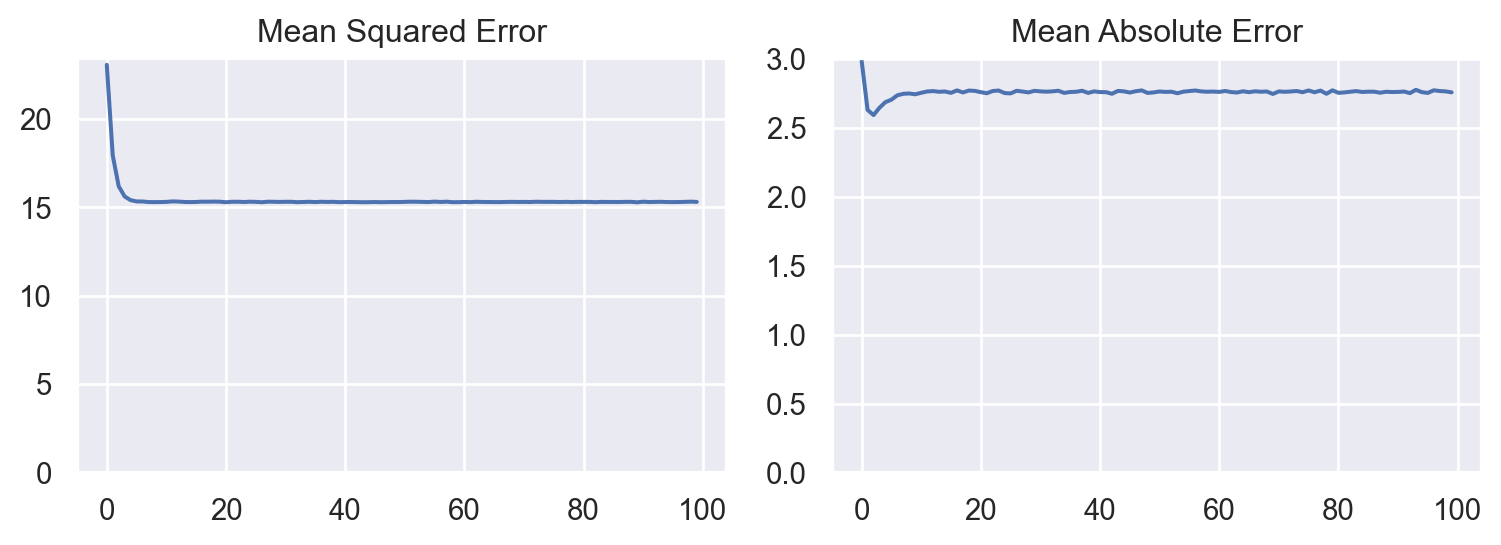
\includegraphics{notebooks/01b-basic-regression_files/figure-pdf/cell-13-output-1.png}

}

\end{figure}

\begin{Shaded}
\begin{Highlighting}[]
\NormalTok{mse, mae }\OperatorTok{=}\NormalTok{ model.evaluate(X\_test, y\_test, verbose }\OperatorTok{=} \DecValTok{0}\NormalTok{)}

\BuiltInTok{print}\NormalTok{(}\SpecialStringTok{f"Mean Squared Error : }\SpecialCharTok{\{}\NormalTok{mse}\SpecialCharTok{:.2f\}}\SpecialStringTok{"}\NormalTok{)}
\BuiltInTok{print}\NormalTok{(}\SpecialStringTok{f"Mean Absolute Error: }\SpecialCharTok{\{}\NormalTok{mae}\SpecialCharTok{:.2f\}}\SpecialStringTok{"}\NormalTok{)}
\end{Highlighting}
\end{Shaded}

\begin{verbatim}
Mean Squared Error : 14.94
Mean Absolute Error: 2.75
\end{verbatim}

\hypertarget{going-deeper-by-using-more-layers}{%
\section{Going Deeper by Using More
Layers}\label{going-deeper-by-using-more-layers}}

As the name suggests, Deep Learning techniques leverages several
intermediate representation of the data before finally decide what value
to assign for any given input. This supports finding complex patterns
that are usually inherent in real world data.

The previous model is modified simply by \texttt{add}ing more
\texttt{Dense} layers and increasing the number of the units. The
\texttt{activation} function in a model is crucial for capturing
non-linearity. The \texttt{relu} activation function is a function that
gives either a positive value or zero which is suprisingly effective for
balancing the trade-offs between finding non-linear pattern and
efficient computation. As each subsequent layer can determine the number
of parameters required through inferring the number of units from the
previous layer, \texttt{input\_shape} is only defined for the first
layer.

\begin{Shaded}
\begin{Highlighting}[]
\NormalTok{model }\OperatorTok{=}\NormalTok{ tf.keras.models.Sequential()}
\NormalTok{model.add(tf.keras.layers.Dense(}\DecValTok{32}\NormalTok{, activation }\OperatorTok{=} \StringTok{"relu"}\NormalTok{, input\_shape }\OperatorTok{=}\NormalTok{ (}\DecValTok{2}\NormalTok{, )))}
\NormalTok{model.add(tf.keras.layers.Dense(}\DecValTok{32}\NormalTok{, activation }\OperatorTok{=} \StringTok{"relu"}\NormalTok{))}
\NormalTok{model.add(tf.keras.layers.Dense(}\DecValTok{1}\NormalTok{))}
\NormalTok{model.}\BuiltInTok{compile}\NormalTok{(optimizer }\OperatorTok{=} \StringTok{"sgd"}\NormalTok{, loss }\OperatorTok{=} \StringTok{"mse"}\NormalTok{, metrics }\OperatorTok{=}\NormalTok{ [}\StringTok{"mae"}\NormalTok{])}

\NormalTok{model.summary()}
\end{Highlighting}
\end{Shaded}

\begin{verbatim}
Model: "sequential_2"
_________________________________________________________________
 Layer (type)                Output Shape              Param #   
=================================================================
 dense_2 (Dense)             (None, 32)                96        
                                                                 
 dense_3 (Dense)             (None, 32)                1056      
                                                                 
 dense_4 (Dense)             (None, 1)                 33        
                                                                 
=================================================================
Total params: 1,185
Trainable params: 1,185
Non-trainable params: 0
_________________________________________________________________
\end{verbatim}

As can be seen in the plots below and the values of MSE and MAE, the
`deeper' version of the model could better capture the inherent trend of
the dataset leading to more superior model than the previous one.

\begin{Shaded}
\begin{Highlighting}[]
\NormalTok{history }\OperatorTok{=}\NormalTok{ model.fit(X\_train, y\_train, epochs }\OperatorTok{=} \DecValTok{100}\NormalTok{, verbose }\OperatorTok{=} \DecValTok{0}\NormalTok{)}

\NormalTok{data }\OperatorTok{=}\NormalTok{ pd.DataFrame(history.history)}
\NormalTok{data }\OperatorTok{=}\NormalTok{ data.reset\_index()}
\NormalTok{data }\OperatorTok{=}\NormalTok{ data.rename(columns }\OperatorTok{=}\NormalTok{ \{}\StringTok{"index"}\NormalTok{:}\StringTok{"epoch"}\NormalTok{, }
                              \StringTok{"loss"}\NormalTok{: }\StringTok{"Mean Squared Error"}\NormalTok{, }
                              \StringTok{"mae"}\NormalTok{: }\StringTok{"Mean Absolute Error"}\NormalTok{\})}
\NormalTok{data }\OperatorTok{=}\NormalTok{ pd.melt(data, }
\NormalTok{               id\_vars }\OperatorTok{=} \StringTok{"epoch"}\NormalTok{, }
\NormalTok{               value\_vars }\OperatorTok{=}\NormalTok{ [}\StringTok{"Mean Squared Error"}\NormalTok{, }\StringTok{"Mean Absolute Error"}\NormalTok{],}
\NormalTok{               var\_name }\OperatorTok{=} \StringTok{"metric"}\NormalTok{,}
\NormalTok{               value\_name }\OperatorTok{=} \StringTok{"value"}\NormalTok{)}

\NormalTok{(}
\NormalTok{    so.Plot(data, x }\OperatorTok{=} \StringTok{"epoch"}\NormalTok{, y }\OperatorTok{=} \StringTok{"value"}\NormalTok{)}
\NormalTok{    .facet(}\StringTok{"metric"}\NormalTok{)}
\NormalTok{    .add(so.Line())}
\NormalTok{    .share(y }\OperatorTok{=} \VariableTok{False}\NormalTok{)}
\NormalTok{    .limit(y }\OperatorTok{=}\NormalTok{ (}\DecValTok{0}\NormalTok{, }\VariableTok{None}\NormalTok{))}
\NormalTok{    .layout(size }\OperatorTok{=}\NormalTok{ (}\DecValTok{8}\NormalTok{, }\DecValTok{3}\NormalTok{))}
\NormalTok{    .label(x }\OperatorTok{=} \StringTok{""}\NormalTok{, y }\OperatorTok{=} \StringTok{""}\NormalTok{)}
\NormalTok{)}
\end{Highlighting}
\end{Shaded}

\begin{figure}[H]

{\centering 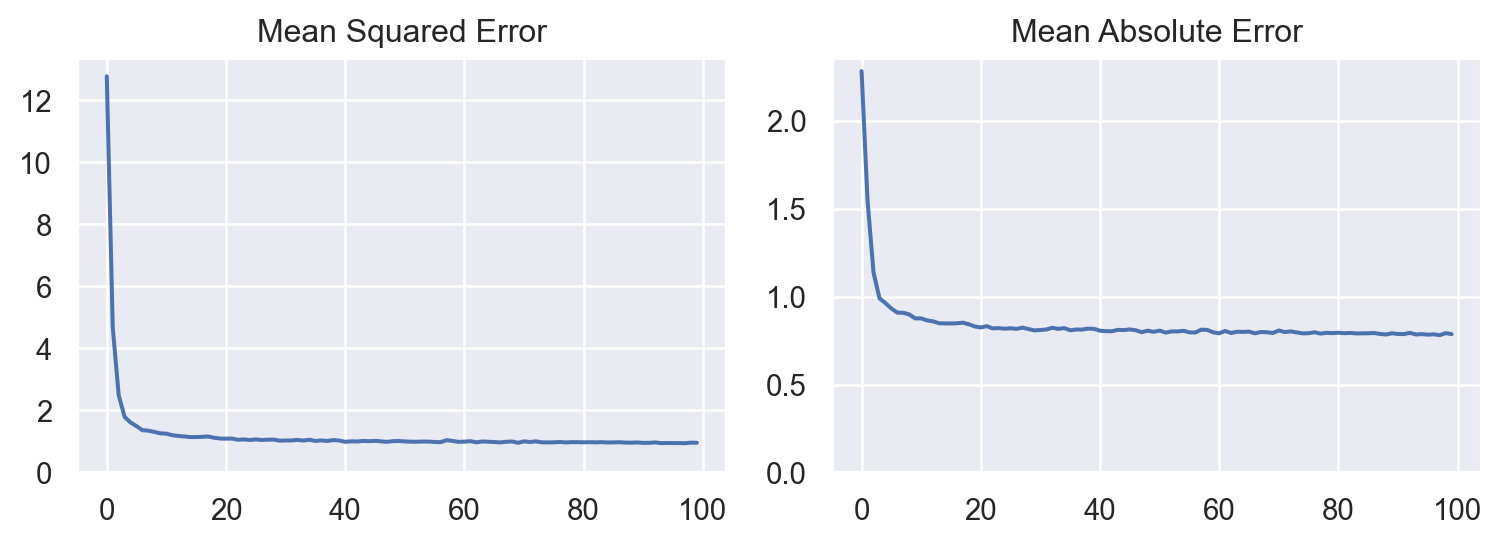
\includegraphics{notebooks/01b-basic-regression_files/figure-pdf/cell-16-output-1.png}

}

\end{figure}

\begin{Shaded}
\begin{Highlighting}[]
\NormalTok{mse, mae }\OperatorTok{=}\NormalTok{ model.evaluate(X\_test, y\_test, verbose }\OperatorTok{=} \DecValTok{0}\NormalTok{)}

\BuiltInTok{print}\NormalTok{(}\SpecialStringTok{f"Mean Squared Error : }\SpecialCharTok{\{}\NormalTok{mse}\SpecialCharTok{:.2f\}}\SpecialStringTok{"}\NormalTok{)}
\BuiltInTok{print}\NormalTok{(}\SpecialStringTok{f"Mean Absolute Error: }\SpecialCharTok{\{}\NormalTok{mae}\SpecialCharTok{:.2f\}}\SpecialStringTok{"}\NormalTok{)}
\end{Highlighting}
\end{Shaded}

\begin{verbatim}
Mean Squared Error : 1.04
Mean Absolute Error: 0.82
\end{verbatim}

\hypertarget{conclusion}{%
\section{Conclusion}\label{conclusion}}

In this post, I demonstrate how to leverage a small subset of TensorFlow
2 capabilities to deal with artificial datasets. Even though here only
includes problems with structured data with well defined problems and
boundaries, Deep Learning model in essence allows anyone to do Machine
Learning for highly unstructured data such as images and texts.

\hypertarget{dealing-with-classification-problems}{%
\chapter{Dealing with Classification
Problems}\label{dealing-with-classification-problems}}

Continuing previous
\href{../post-06-tensorflow-regression-basics}{post}, this demo will
show you how to leverage TensorFlow 2 (TF2) for dealing with
classification problems. An additional technique to tune hyperparameter
(which in this case is the number of epochs) is presented here. Similar
to the previous demo, the data for illustration is randomly generated
using \texttt{numpy} library.

The objective of this demo is to show you the main elements of working
with a TF2 model to tackle classification problems.

The setup includes importing important libraries (\texttt{tensorflow},
\texttt{numpy}, and \texttt{matplotlib.pyplot}), freeing memory from old
models/layers (if any) and setting the seed for random number generator.

\begin{Shaded}
\begin{Highlighting}[]
\ImportTok{import}\NormalTok{ tensorflow }\ImportTok{as}\NormalTok{ tf}
\ImportTok{import}\NormalTok{ numpy }\ImportTok{as}\NormalTok{ np}
\ImportTok{import}\NormalTok{ matplotlib.pyplot }\ImportTok{as}\NormalTok{ plt}
\end{Highlighting}
\end{Shaded}

\begin{Shaded}
\begin{Highlighting}[]
\NormalTok{tf.keras.backend.clear\_session()}
\NormalTok{tf.keras.utils.set\_random\_seed(}\DecValTok{123}\NormalTok{)}
\end{Highlighting}
\end{Shaded}

\hypertarget{generate-random-data-1}{%
\section{Generate Random Data}\label{generate-random-data-1}}

For this use case, I genereated two classes of data based on
multivariate normal distribution with specified means and covariance
matrices. Both values are determined arbitrarily.

\begin{Shaded}
\begin{Highlighting}[]
\CommentTok{\# random data generation}
\NormalTok{SAMPLE\_SIZE }\OperatorTok{=} \DecValTok{1500}

\NormalTok{class\_1 }\OperatorTok{=}\NormalTok{ np.random.multivariate\_normal(}
\NormalTok{    mean }\OperatorTok{=}\NormalTok{ [}\DecValTok{0}\NormalTok{, }\DecValTok{2}\NormalTok{],}
\NormalTok{    cov  }\OperatorTok{=}\NormalTok{ [[}\DecValTok{1}\NormalTok{, }\FloatTok{0.1}\NormalTok{], [}\FloatTok{0.1}\NormalTok{, }\DecValTok{1}\NormalTok{]],}
\NormalTok{    size }\OperatorTok{=}\NormalTok{ SAMPLE\_SIZE}
\NormalTok{)}

\NormalTok{class\_2 }\OperatorTok{=}\NormalTok{ np.random.multivariate\_normal(}
\NormalTok{    mean }\OperatorTok{=}\NormalTok{ [}\DecValTok{2}\NormalTok{, }\DecValTok{0}\NormalTok{],}
\NormalTok{    cov  }\OperatorTok{=}\NormalTok{ [[}\DecValTok{1}\NormalTok{, }\FloatTok{0.1}\NormalTok{], [}\FloatTok{0.1}\NormalTok{, }\DecValTok{1}\NormalTok{]],}
\NormalTok{    size }\OperatorTok{=}\NormalTok{ SAMPLE\_SIZE}
\NormalTok{)}

\CommentTok{\# append both classes}
\NormalTok{X }\OperatorTok{=}\NormalTok{ np.concatenate([class\_1, class\_2])}
\NormalTok{X }\OperatorTok{=}\NormalTok{ X.astype(}\StringTok{"float32"}\NormalTok{)}

\NormalTok{y }\OperatorTok{=}\NormalTok{ np.concatenate([np.zeros((SAMPLE\_SIZE, }\DecValTok{1}\NormalTok{)), np.ones((SAMPLE\_SIZE, }\DecValTok{1}\NormalTok{))])}
\NormalTok{y }\OperatorTok{=}\NormalTok{ y.astype(}\StringTok{"int"}\NormalTok{)}

\NormalTok{X.shape, y.shape}
\end{Highlighting}
\end{Shaded}

\begin{verbatim}
((3000, 2), (3000, 1))
\end{verbatim}

As there are only two variables within the data, making sense of it is
easier as we only requires a scatter plot to see how data is dispersed
along x and y axes. As you can see from the figure below, there is an
area where points from class 1 and class 2 overlap.

\begin{Shaded}
\begin{Highlighting}[]
\NormalTok{plt.scatter(X[:, }\DecValTok{0}\NormalTok{], X[:, }\DecValTok{1}\NormalTok{], c }\OperatorTok{=}\NormalTok{ y[:, }\DecValTok{0}\NormalTok{], alpha }\OperatorTok{=} \FloatTok{.2}\NormalTok{)}
\NormalTok{plt.show()}
\end{Highlighting}
\end{Shaded}

\begin{figure}[H]

{\centering 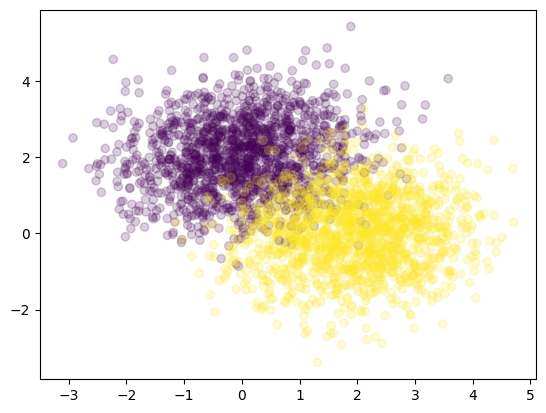
\includegraphics{notebooks/01c-basic-classification_files/figure-pdf/cell-5-output-1.png}

}

\end{figure}

\hypertarget{slice-the-data}{%
\section{Slice the Data}\label{slice-the-data}}

To help slicing two python variables with the same length (\texttt{X}
and \texttt{y}), I created a vector of data indices where the order is
shuffled. This then server as a reference to determine which points
belong to which datasets (training, validation, or testing).

I split the data into train and test datasets (80\% and 20\%), before
splitting the train dataset further for hyperparameter tuning into
partial train and validation (80\% and 20\%).

\begin{Shaded}
\begin{Highlighting}[]
\CommentTok{\# define randomized indices for splitting}
\NormalTok{indices }\OperatorTok{=}\NormalTok{ np.arange(SAMPLE\_SIZE }\OperatorTok{*} \DecValTok{2}\NormalTok{)}
\NormalTok{np.random.shuffle(indices)}

\CommentTok{\# split data into \textasciigrave{}train\textasciigrave{} and \textasciigrave{}test datasets\textasciigrave{}}
\NormalTok{split\_locaction }\OperatorTok{=} \BuiltInTok{round}\NormalTok{(SAMPLE\_SIZE }\OperatorTok{*} \FloatTok{.8}\NormalTok{)}

\NormalTok{X\_train }\OperatorTok{=}\NormalTok{ X[indices[:split\_locaction]]}
\NormalTok{y\_train }\OperatorTok{=}\NormalTok{ y[indices[:split\_locaction]]}

\NormalTok{X\_test }\OperatorTok{=}\NormalTok{ X[indices[split\_locaction:]]}
\NormalTok{y\_test }\OperatorTok{=}\NormalTok{ y[indices[split\_locaction:]]}

\NormalTok{X\_train.shape, y\_train.shape, X\_test.shape, y\_test.shape}
\end{Highlighting}
\end{Shaded}

\begin{verbatim}
((1200, 2), (1200, 1), (1800, 2), (1800, 1))
\end{verbatim}

\begin{Shaded}
\begin{Highlighting}[]
\CommentTok{\# split train data into \textasciigrave{}partial\textasciigrave{} and \textasciigrave{}validation\textasciigrave{} for hyperparameter tuning}
\NormalTok{split\_locaction }\OperatorTok{=} \BuiltInTok{round}\NormalTok{(}\BuiltInTok{len}\NormalTok{(X\_train) }\OperatorTok{*} \FloatTok{.8}\NormalTok{)}

\NormalTok{partial\_X\_train }\OperatorTok{=}\NormalTok{ X\_train[:split\_locaction]}
\NormalTok{partial\_y\_train }\OperatorTok{=}\NormalTok{ y\_train[:split\_locaction]}

\NormalTok{X\_val }\OperatorTok{=}\NormalTok{ X\_train[split\_locaction:]}
\NormalTok{y\_val }\OperatorTok{=}\NormalTok{ y\_train[split\_locaction:]}

\NormalTok{partial\_X\_train.shape, partial\_y\_train.shape, X\_val.shape, y\_val.shape}
\end{Highlighting}
\end{Shaded}

\begin{verbatim}
((960, 2), (960, 1), (240, 2), (240, 1))
\end{verbatim}

\hypertarget{hyperparameter-optimization}{%
\section{Hyperparameter
Optimization}\label{hyperparameter-optimization}}

Hyperparameter optimization or tuning can be applied to any parameters
controlling the behaviours of the machine learning algorithm which are
not learned during training. In doing so, we need to separate the test
data and leverage two subsets of training data instead. Otherwise, there
might be any leak of information from the `unseen data' which might
alter the result of the trained algorithm giving it the capability to
perform better on the test dataset. This opposes the idea of ML model
that should be able to do well given unknown input, which, in this case
is represented as test dataset.

The hyperparameter to be tuned is the simple one, in this case number of
epochs.The process includes training a network with simplifed
architecture, then analyses the performance of the network throughout
the training. The optimal number of epochs is decided based on how
accuracy and loss values moves throughout time.

The actual workflow for creating the model, compiling its optimizer,
loss function, and metrics, and fitting it to the data is similar to
what you can see from the previous demo. The difference here is that I
did not use \texttt{model.add} method to put a layer in the model.
Instead, I gave a list of several \texttt{Dense} layers as an argument
when instantiating a \texttt{Sequential} model. In addition, the number
of units in each layer is a reduced one (we will increase it when
training with full train data). I also set the learning rate for the
\texttt{SGD} optimizer into 0.005.

\begin{Shaded}
\begin{Highlighting}[]
\NormalTok{model }\OperatorTok{=}\NormalTok{ tf.keras.models.Sequential([}
\NormalTok{    tf.keras.layers.Dense(}\DecValTok{8}\NormalTok{, input\_shape }\OperatorTok{=}\NormalTok{ (}\DecValTok{2}\NormalTok{,), activation }\OperatorTok{=} \StringTok{"relu"}\NormalTok{),}
\NormalTok{    tf.keras.layers.Dense(}\DecValTok{8}\NormalTok{, activation }\OperatorTok{=} \StringTok{"relu"}\NormalTok{),}
\NormalTok{    tf.keras.layers.Dense(}\DecValTok{1}\NormalTok{, activation }\OperatorTok{=} \StringTok{"sigmoid"}\NormalTok{)}
\NormalTok{])}

\NormalTok{model.}\BuiltInTok{compile}\NormalTok{(optimizer }\OperatorTok{=}\NormalTok{ tf.keras.optimizers.SGD(learning\_rate }\OperatorTok{=} \FloatTok{0.005}\NormalTok{), }
\NormalTok{              loss }\OperatorTok{=} \StringTok{"binary\_crossentropy"}\NormalTok{,}
\NormalTok{              metrics }\OperatorTok{=}\NormalTok{ [}\StringTok{"accuracy"}\NormalTok{])}

\NormalTok{history }\OperatorTok{=}\NormalTok{ model.fit(partial\_X\_train, }
\NormalTok{                    partial\_y\_train, }
\NormalTok{                    validation\_data}\OperatorTok{=}\NormalTok{(X\_val, y\_val), }
\NormalTok{                    epochs }\OperatorTok{=} \DecValTok{1000}\NormalTok{, }
\NormalTok{                    verbose }\OperatorTok{=} \DecValTok{0}\NormalTok{)}
\end{Highlighting}
\end{Shaded}

The model is fitted using the \texttt{partial\_X\_train} and
\texttt{partial\_y\_train} with a set of validation data. By using
validation data, we might observe how the performance of the model
throughout training.

Below, we can see the values of training and validation accuracy and
loss given a certain training epoch. Because of the values for the
validation seems to resemble training values, it can be inferred that
the model does not overfit. Overfitting may cause the training accuracy
to be significantly higher than validation accuracy and training loss to
be significantly lower than validation loss.

\begin{Shaded}
\begin{Highlighting}[]
\CommentTok{\# Plot the training results}
\NormalTok{accuracy     }\OperatorTok{=}\NormalTok{ history.history[}\StringTok{\textquotesingle{}accuracy\textquotesingle{}}\NormalTok{]}
\NormalTok{val\_accuracy }\OperatorTok{=}\NormalTok{ history.history[}\StringTok{\textquotesingle{}val\_accuracy\textquotesingle{}}\NormalTok{]}
\NormalTok{epochs       }\OperatorTok{=} \BuiltInTok{range}\NormalTok{(}\BuiltInTok{len}\NormalTok{(accuracy))}

\NormalTok{plt.plot(epochs, accuracy, }\StringTok{\textquotesingle{}r\textquotesingle{}}\NormalTok{, label}\OperatorTok{=}\StringTok{\textquotesingle{}Training accuracy\textquotesingle{}}\NormalTok{)}
\NormalTok{plt.plot(epochs, val\_accuracy, }\StringTok{\textquotesingle{}b\textquotesingle{}}\NormalTok{, label}\OperatorTok{=}\StringTok{\textquotesingle{}Validation accuracy\textquotesingle{}}\NormalTok{)}
\NormalTok{plt.title(}\StringTok{\textquotesingle{}Training and validation accuracy\textquotesingle{}}\NormalTok{)}
\NormalTok{plt.ylim(ymin}\OperatorTok{=}\DecValTok{0}\NormalTok{)}
\NormalTok{plt.legend()}
\NormalTok{plt.show()}
\end{Highlighting}
\end{Shaded}

\begin{figure}[H]

{\centering 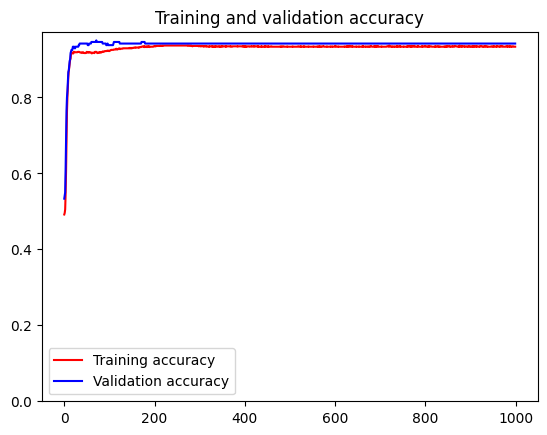
\includegraphics{notebooks/01c-basic-classification_files/figure-pdf/cell-9-output-1.png}

}

\end{figure}

\begin{Shaded}
\begin{Highlighting}[]
\CommentTok{\# Plot the training results}
\NormalTok{loss     }\OperatorTok{=}\NormalTok{ history.history[}\StringTok{\textquotesingle{}loss\textquotesingle{}}\NormalTok{]}
\NormalTok{val\_loss }\OperatorTok{=}\NormalTok{ history.history[}\StringTok{\textquotesingle{}val\_loss\textquotesingle{}}\NormalTok{]}
\NormalTok{epochs   }\OperatorTok{=} \BuiltInTok{range}\NormalTok{(}\BuiltInTok{len}\NormalTok{(accuracy))}

\NormalTok{plt.plot(epochs, loss, }\StringTok{\textquotesingle{}r\textquotesingle{}}\NormalTok{, label}\OperatorTok{=}\StringTok{\textquotesingle{}Training Loss\textquotesingle{}}\NormalTok{)}
\NormalTok{plt.plot(epochs, val\_loss, }\StringTok{\textquotesingle{}b\textquotesingle{}}\NormalTok{, label}\OperatorTok{=}\StringTok{\textquotesingle{}Validation Loss\textquotesingle{}}\NormalTok{)}
\NormalTok{plt.title(}\StringTok{\textquotesingle{}Training and validation loss\textquotesingle{}}\NormalTok{)}
\NormalTok{plt.ylim(ymin}\OperatorTok{=}\DecValTok{0}\NormalTok{)}
\NormalTok{plt.legend()}
\NormalTok{plt.show()}
\end{Highlighting}
\end{Shaded}

\begin{figure}[H]

{\centering \includegraphics{notebooks/01c-basic-classification_files/figure-pdf/cell-10-output-1.png}

}

\end{figure}

\hypertarget{fitting-with-full-training-data}{%
\section{Fitting with Full Training
Data}\label{fitting-with-full-training-data}}

After observing how the simplified model performs, we were able to
decide at which epoch we want to stop training our model. In this case,
we selected 175 as the subsequent epochs does not give improvement to
the model (the loss seemed to stop decreasing). We then could fit our
model with full training data and increase the number of units for each
\texttt{Dense} layer.

\begin{Shaded}
\begin{Highlighting}[]
\NormalTok{model }\OperatorTok{=}\NormalTok{ tf.keras.models.Sequential([}
\NormalTok{    tf.keras.layers.Dense(}\DecValTok{64}\NormalTok{, input\_shape }\OperatorTok{=}\NormalTok{ (}\DecValTok{2}\NormalTok{,), activation }\OperatorTok{=} \StringTok{"relu"}\NormalTok{),}
\NormalTok{    tf.keras.layers.Dense(}\DecValTok{64}\NormalTok{, activation }\OperatorTok{=} \StringTok{"relu"}\NormalTok{),}
\NormalTok{    tf.keras.layers.Dense(}\DecValTok{1}\NormalTok{, activation }\OperatorTok{=} \StringTok{"sigmoid"}\NormalTok{)}
\NormalTok{])}

\NormalTok{model.}\BuiltInTok{compile}\NormalTok{(optimizer }\OperatorTok{=}\NormalTok{ tf.keras.optimizers.SGD(learning\_rate }\OperatorTok{=} \FloatTok{0.005}\NormalTok{), }
\NormalTok{              loss }\OperatorTok{=} \StringTok{"binary\_crossentropy"}\NormalTok{,}
\NormalTok{              metrics }\OperatorTok{=}\NormalTok{ [}\StringTok{"accuracy"}\NormalTok{])}

\NormalTok{history }\OperatorTok{=}\NormalTok{ model.fit(X\_train, y\_train, epochs }\OperatorTok{=} \DecValTok{175}\NormalTok{, verbose }\OperatorTok{=} \DecValTok{0}\NormalTok{)}
\end{Highlighting}
\end{Shaded}

Next, we see how the model classifies each data point from the graph
below.

\begin{Shaded}
\begin{Highlighting}[]
\NormalTok{y\_pred }\OperatorTok{=}\NormalTok{ model.predict(X\_test, verbose }\OperatorTok{=} \DecValTok{0}\NormalTok{)}

\NormalTok{plt.scatter(X\_test[:, }\DecValTok{0}\NormalTok{], X\_test[:, }\DecValTok{1}\NormalTok{], c }\OperatorTok{=}\NormalTok{ y\_pred[:, }\DecValTok{0}\NormalTok{] }\OperatorTok{\textgreater{}} \FloatTok{.5}\NormalTok{, alpha }\OperatorTok{=} \FloatTok{.3}\NormalTok{)}
\NormalTok{plt.show()}
\end{Highlighting}
\end{Shaded}

\begin{figure}[H]

{\centering 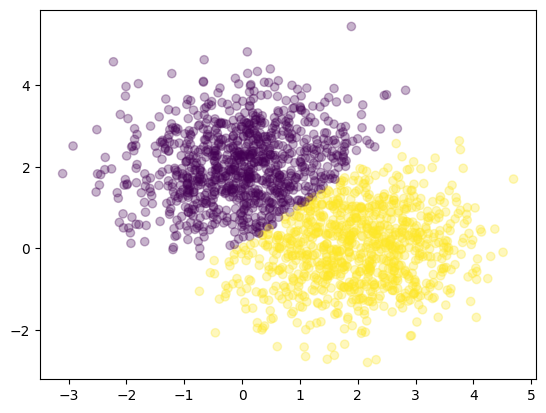
\includegraphics{notebooks/01c-basic-classification_files/figure-pdf/cell-12-output-1.png}

}

\end{figure}

We could also \texttt{evaluate} the performance on the test dataset. The
model can reach more than 80\% accuracy.

\begin{Shaded}
\begin{Highlighting}[]
\NormalTok{loss, accuracy }\OperatorTok{=}\NormalTok{ model.evaluate(X\_test, y\_test, verbose }\OperatorTok{=} \DecValTok{0}\NormalTok{)}

\BuiltInTok{print}\NormalTok{(}\SpecialStringTok{f"Loss    : }\SpecialCharTok{\{}\NormalTok{loss}\SpecialCharTok{:.3f\}}\SpecialStringTok{"}\NormalTok{)}
\BuiltInTok{print}\NormalTok{(}\SpecialStringTok{f"Accuracy: }\SpecialCharTok{\{}\NormalTok{accuracy}\SpecialCharTok{:.3f\}}\SpecialStringTok{"}\NormalTok{)}
\end{Highlighting}
\end{Shaded}

\begin{verbatim}
Loss    : 0.176
Accuracy: 0.926
\end{verbatim}

\hypertarget{conclusion-1}{%
\section{Conclusion}\label{conclusion-1}}

In this post, we continue our demonstration of TensorFlow 2 with
classification problems. The model successfully achieve a decent
accuracy score for this simple case. Additionally, we have touched the
concept of hyperparameter tuning which is essential for doing machine
learning.

\part{{Use Cases of TensorFlow 2}}

\hypertarget{mnist}{%
\chapter{MNIST}\label{mnist}}

\begin{Shaded}
\begin{Highlighting}[]
\ImportTok{import}\NormalTok{ numpy }\ImportTok{as}\NormalTok{ np}
\ImportTok{from}\NormalTok{ tensorflow.keras.datasets }\ImportTok{import}\NormalTok{ mnist}
\ImportTok{from}\NormalTok{ tensorflow.keras.utils }\ImportTok{import}\NormalTok{ to\_categorical}
\ImportTok{from}\NormalTok{ tensorflow.keras }\ImportTok{import}\NormalTok{ models, layers, optimizers, backend}
\end{Highlighting}
\end{Shaded}

\begin{Shaded}
\begin{Highlighting}[]
\CommentTok{\# load dataset}
\NormalTok{(train\_images, train\_labels), (test\_images, test\_labels) }\OperatorTok{=}\NormalTok{ mnist.load\_data()}

\NormalTok{train\_labels }\OperatorTok{=}\NormalTok{ to\_categorical(train\_labels)}
\NormalTok{test\_labels }\OperatorTok{=}\NormalTok{ to\_categorical(test\_labels)}

\CommentTok{\# transform image data}
\NormalTok{train\_images }\OperatorTok{=}\NormalTok{ train\_images.reshape((}\DecValTok{60000}\NormalTok{, }\DecValTok{28} \OperatorTok{*} \DecValTok{28}\NormalTok{)) }\OperatorTok{/} \DecValTok{255}
\NormalTok{test\_images }\OperatorTok{=}\NormalTok{ test\_images.reshape((}\DecValTok{10000}\NormalTok{, }\DecValTok{28} \OperatorTok{*} \DecValTok{28}\NormalTok{)) }\OperatorTok{/} \DecValTok{255}

\NormalTok{train\_images.shape, train\_labels.shape, test\_images.shape, test\_labels.shape}
\end{Highlighting}
\end{Shaded}

\begin{Shaded}
\begin{Highlighting}[]
\KeywordTok{def}\NormalTok{ explore(train\_images, }
\NormalTok{            train\_labels, }
\NormalTok{            test\_images, }
\NormalTok{            test\_labels,}
\NormalTok{            label\_count,}
\NormalTok{            neuron\_count,}
\NormalTok{            learning\_rate,}
\NormalTok{            momentum):}

    \CommentTok{\# define ann architecture}
\NormalTok{    model }\OperatorTok{=}\NormalTok{ models.Sequential()}
\NormalTok{    model.add(layers.Dense(neuron\_count, activation }\OperatorTok{=} \StringTok{"relu"}\NormalTok{, input\_shape }\OperatorTok{=}\NormalTok{ (}\DecValTok{28} \OperatorTok{*} \DecValTok{28}\NormalTok{,)))}
\NormalTok{    model.add(layers.Dense(label\_count, activation }\OperatorTok{=} \StringTok{"softmax"}\NormalTok{))}

    \CommentTok{\# define optimizer, loss function, and metrics}
\NormalTok{    optimizer }\OperatorTok{=}\NormalTok{ optimizers.RMSprop(learning\_rate }\OperatorTok{=}\NormalTok{ learning\_rate, momentum }\OperatorTok{=}\NormalTok{ momentum)}

\NormalTok{    model.}\BuiltInTok{compile}\NormalTok{(optimizer }\OperatorTok{=}\NormalTok{ optimizer,}
\NormalTok{                  loss }\OperatorTok{=} \StringTok{"categorical\_crossentropy"}\NormalTok{,}
\NormalTok{                  metrics }\OperatorTok{=}\NormalTok{ [}\StringTok{"accuracy"}\NormalTok{])}

    \CommentTok{\# train ann model}
\NormalTok{    history }\OperatorTok{=}\NormalTok{ model.fit(train\_images, train\_labels, epochs }\OperatorTok{=} \DecValTok{20}\NormalTok{, batch\_size }\OperatorTok{=} \DecValTok{64}\NormalTok{, verbose }\OperatorTok{=} \DecValTok{0}\NormalTok{)}

    \CommentTok{\# evaluate ann model}
\NormalTok{    test\_loss, test\_acc }\OperatorTok{=}\NormalTok{ model.evaluate(test\_images, test\_labels, verbose }\OperatorTok{=} \DecValTok{0}\NormalTok{)}

    \ControlFlowTok{return}\NormalTok{ history, test\_loss, test\_acc}
\end{Highlighting}
\end{Shaded}

\begin{Shaded}
\begin{Highlighting}[]
\CommentTok{\# set hyperparameters}
\NormalTok{learning\_rates }\OperatorTok{=}\NormalTok{ np.logspace(}\OperatorTok{{-}}\DecValTok{1}\NormalTok{, }\OperatorTok{{-}}\DecValTok{4}\NormalTok{, }\DecValTok{5}\NormalTok{)}
\NormalTok{momentums }\OperatorTok{=}\NormalTok{ np.logspace(}\OperatorTok{{-}}\DecValTok{1}\NormalTok{, }\OperatorTok{{-}}\DecValTok{4}\NormalTok{, }\DecValTok{5}\NormalTok{)}
\NormalTok{neuron\_counts }\OperatorTok{=} \DecValTok{2} \OperatorTok{**}\NormalTok{ np.arange(}\DecValTok{7}\NormalTok{, }\DecValTok{12}\NormalTok{)}

\NormalTok{hyparameters\_list }\OperatorTok{=}\NormalTok{ []}
\ControlFlowTok{for}\NormalTok{ learning\_rate }\KeywordTok{in}\NormalTok{ learning\_rates:}
    \ControlFlowTok{for}\NormalTok{ momentum }\KeywordTok{in}\NormalTok{ momentums:}
        \ControlFlowTok{for}\NormalTok{ neuron\_count }\KeywordTok{in}\NormalTok{ neuron\_counts:}
\NormalTok{            hyparameters\_list.append(\{}
                \StringTok{"learning\_rate"}\NormalTok{: learning\_rate,}
                \StringTok{"momentum"}\NormalTok{: momentum,}
                \StringTok{"neuron\_count"}\NormalTok{: neuron\_count}
\NormalTok{            \})}
\end{Highlighting}
\end{Shaded}

\begin{Shaded}
\begin{Highlighting}[]
\NormalTok{output }\OperatorTok{=}\NormalTok{ []}
\ControlFlowTok{for}\NormalTok{ hyparameters }\KeywordTok{in}\NormalTok{ hyparameters\_list:}
\NormalTok{    history, test\_loss, test\_acc }\OperatorTok{=}\NormalTok{ explore(}
\NormalTok{        train\_images,}
\NormalTok{        train\_labels,}
\NormalTok{        test\_images,}
\NormalTok{        test\_labels,}
\NormalTok{        label\_count }\OperatorTok{=} \DecValTok{10}\NormalTok{,}
\NormalTok{        learning\_rate }\OperatorTok{=}\NormalTok{ hyparameters[}\StringTok{"learning\_rate"}\NormalTok{],}
\NormalTok{        momentum }\OperatorTok{=}\NormalTok{ hyparameters[}\StringTok{"momentum"}\NormalTok{],}
\NormalTok{        neuron\_count }\OperatorTok{=}\NormalTok{ hyparameters[}\StringTok{"neuron\_count"}\NormalTok{]}
\NormalTok{    )}
    
\NormalTok{    output.append(\{}
        \StringTok{"history"}\NormalTok{: history,}
        \StringTok{"test\_loss"}\NormalTok{: test\_loss, }
        \StringTok{"test\_acc"}\NormalTok{: test\_acc,}
        \StringTok{"hyperparameters"}\NormalTok{: hyparameters}
\NormalTok{    \})}
\NormalTok{    backend.clear\_session()}

    \BuiltInTok{print}\NormalTok{(}\SpecialStringTok{f"A model is trained with hyperparameters of }\SpecialCharTok{\{}\NormalTok{hyparameters}\SpecialCharTok{\}}\SpecialStringTok{"}\NormalTok{)}
\end{Highlighting}
\end{Shaded}

\hypertarget{imdb}{%
\chapter{IMDB}\label{imdb}}

\begin{Shaded}
\begin{Highlighting}[]
\ImportTok{import}\NormalTok{ matplotlib.pyplot }\ImportTok{as}\NormalTok{ plt}
\ImportTok{import}\NormalTok{ numpy }\ImportTok{as}\NormalTok{ np}
\ImportTok{from}\NormalTok{ tensorflow.keras.datasets }\ImportTok{import}\NormalTok{ imdb}
\ImportTok{from}\NormalTok{ tensorflow.keras }\ImportTok{import}\NormalTok{ models, layers, optimizers, backend}
\end{Highlighting}
\end{Shaded}

\begin{Shaded}
\begin{Highlighting}[]
\CommentTok{\# load dataset}
\NormalTok{num\_words }\OperatorTok{=} \DecValTok{10000}

\NormalTok{(train\_data, train\_labels), (test\_data, test\_labels) }\OperatorTok{=}\NormalTok{ imdb.load\_data(num\_words }\OperatorTok{=}\NormalTok{ num\_words)}

\NormalTok{train\_data.shape, train\_labels.shape, test\_data.shape, test\_labels.shape}
\end{Highlighting}
\end{Shaded}

\begin{Shaded}
\begin{Highlighting}[]
\CommentTok{\# preprocess}
\NormalTok{X\_train }\OperatorTok{=}\NormalTok{ np.zeros(shape }\OperatorTok{=}\NormalTok{ (}\BuiltInTok{len}\NormalTok{(train\_data), num\_words), dtype }\OperatorTok{=} \BuiltInTok{float}\NormalTok{)}
\NormalTok{X\_test }\OperatorTok{=}\NormalTok{ np.zeros(shape }\OperatorTok{=}\NormalTok{ (}\BuiltInTok{len}\NormalTok{(test\_data), num\_words), dtype }\OperatorTok{=} \BuiltInTok{float}\NormalTok{)}

\ControlFlowTok{for}\NormalTok{ i, seq }\KeywordTok{in} \BuiltInTok{enumerate}\NormalTok{(train\_data):}
\NormalTok{    X\_train[i, seq] }\OperatorTok{=} \FloatTok{1.}

\ControlFlowTok{for}\NormalTok{ i, seq }\KeywordTok{in} \BuiltInTok{enumerate}\NormalTok{(test\_data):}
\NormalTok{    X\_test[i, seq] }\OperatorTok{=} \FloatTok{1.}

\NormalTok{y\_train }\OperatorTok{=}\NormalTok{ train\_labels.astype(}\BuiltInTok{float}\NormalTok{)}
\NormalTok{y\_test }\OperatorTok{=}\NormalTok{ test\_labels.astype(}\BuiltInTok{float}\NormalTok{)}

\BuiltInTok{print}\NormalTok{(X\_train.shape, y\_train.shape, X\_test.shape, y\_test.shape)}
\end{Highlighting}
\end{Shaded}

\begin{Shaded}
\begin{Highlighting}[]
\NormalTok{partial\_X\_train }\OperatorTok{=}\NormalTok{ X\_train[:}\DecValTok{12500}\NormalTok{]}
\NormalTok{partial\_y\_train }\OperatorTok{=}\NormalTok{ y\_train[:}\DecValTok{12500}\NormalTok{]}
\NormalTok{X\_val }\OperatorTok{=}\NormalTok{ X\_train[}\DecValTok{12500}\NormalTok{:]}
\NormalTok{y\_val }\OperatorTok{=}\NormalTok{ y\_train[}\DecValTok{12500}\NormalTok{:]}
\end{Highlighting}
\end{Shaded}

\begin{Shaded}
\begin{Highlighting}[]
\KeywordTok{def}\NormalTok{ explore(X\_train, }
\NormalTok{            y\_train,}
\NormalTok{            X\_val,}
\NormalTok{            y\_val,}
\NormalTok{            n\_units,}
\NormalTok{            n\_layers,}
\NormalTok{            activation,}
\NormalTok{            learning\_rate,}
\NormalTok{            momentum):}
    
    \CommentTok{\# define ann architecture}
\NormalTok{    model }\OperatorTok{=}\NormalTok{ models.Sequential()}
    \ControlFlowTok{for}\NormalTok{ i }\KeywordTok{in} \BuiltInTok{range}\NormalTok{(n\_layers):}
\NormalTok{        model.add(layers.Dense(n\_units, activation }\OperatorTok{=}\NormalTok{ activation))}
\NormalTok{    model.add(layers.Dense(}\DecValTok{1}\NormalTok{, activation }\OperatorTok{=} \StringTok{"sigmoid"}\NormalTok{))}

    \CommentTok{\# define optimizer, loss function, and metrics}
\NormalTok{    optimizer }\OperatorTok{=}\NormalTok{ optimizers.RMSprop(learning\_rate }\OperatorTok{=}\NormalTok{ learning\_rate, momentum }\OperatorTok{=}\NormalTok{ momentum)}


    \CommentTok{\# train ann model}
\NormalTok{    model.build(input\_shape }\OperatorTok{=}\NormalTok{ (}\DecValTok{10000}\NormalTok{,))}
\NormalTok{    model.}\BuiltInTok{compile}\NormalTok{(optimizer }\OperatorTok{=}\NormalTok{ optimizer, loss }\OperatorTok{=} \StringTok{"binary\_crossentropy"}\NormalTok{, metrics }\OperatorTok{=}\NormalTok{ [}\StringTok{"accuracy"}\NormalTok{])}
\NormalTok{    model.fit(X\_train, y\_train, epochs }\OperatorTok{=} \DecValTok{20}\NormalTok{, batch\_size }\OperatorTok{=} \DecValTok{64}\NormalTok{, verbose }\OperatorTok{=} \DecValTok{0}\NormalTok{)}

    \CommentTok{\# evaluate ann model}
\NormalTok{    val\_loss, val\_acc }\OperatorTok{=}\NormalTok{ model.evaluate(X\_val, y\_val, verbose }\OperatorTok{=} \DecValTok{0}\NormalTok{)}

    \ControlFlowTok{return}\NormalTok{ val\_loss, val\_acc}
\end{Highlighting}
\end{Shaded}

\begin{Shaded}
\begin{Highlighting}[]
\CommentTok{\# set hyperparameters}
\NormalTok{learning\_rate\_list  }\OperatorTok{=}\NormalTok{ np.logspace(}\OperatorTok{{-}}\DecValTok{2}\NormalTok{, }\OperatorTok{{-}}\DecValTok{4}\NormalTok{, }\DecValTok{5}\NormalTok{)}
\NormalTok{momentum\_list       }\OperatorTok{=}\NormalTok{ np.linspace(}\FloatTok{0.1}\NormalTok{, }\FloatTok{0.9}\NormalTok{, }\DecValTok{5}\NormalTok{)}
\NormalTok{n\_unit\_list         }\OperatorTok{=}\NormalTok{ [}\DecValTok{32}\NormalTok{, }\DecValTok{64}\NormalTok{]}
\NormalTok{n\_hidden\_layer\_list }\OperatorTok{=}\NormalTok{ [}\DecValTok{1}\NormalTok{, }\DecValTok{3}\NormalTok{]}
\NormalTok{activation\_list     }\OperatorTok{=}\NormalTok{ [}\StringTok{"relu"}\NormalTok{, }\StringTok{"tanh"}\NormalTok{]}

\NormalTok{param\_list }\OperatorTok{=}\NormalTok{ []}
\ControlFlowTok{for}\NormalTok{ learning\_rate }\KeywordTok{in}\NormalTok{ learning\_rate\_list:}
    \ControlFlowTok{for}\NormalTok{ momentum }\KeywordTok{in}\NormalTok{ momentum\_list:}
        \ControlFlowTok{for}\NormalTok{ n\_units }\KeywordTok{in}\NormalTok{ n\_unit\_list:}
            \ControlFlowTok{for}\NormalTok{ n\_layers }\KeywordTok{in}\NormalTok{ n\_hidden\_layer\_list:}
                \ControlFlowTok{for}\NormalTok{ activation }\KeywordTok{in}\NormalTok{ activation\_list:}
\NormalTok{                    param\_list.append(\{}
                        \StringTok{"learning\_rate"}\NormalTok{: learning\_rate,}
                        \StringTok{"momentum"}\NormalTok{: momentum,}
                        \StringTok{"n\_units"}\NormalTok{: n\_units,}
                        \StringTok{"n\_layers"}\NormalTok{: n\_layers,}
                        \StringTok{"activation"}\NormalTok{: activation}
\NormalTok{                    \})}
\end{Highlighting}
\end{Shaded}

\begin{Shaded}
\begin{Highlighting}[]
\NormalTok{results }\OperatorTok{=}\NormalTok{ []}
\ControlFlowTok{for}\NormalTok{ params }\KeywordTok{in}\NormalTok{ param\_list:}
\NormalTok{    val\_loss, val\_acc }\OperatorTok{=}\NormalTok{ explore(}
\NormalTok{        partial\_X\_train, }
\NormalTok{        partial\_y\_train,}
\NormalTok{        X\_val,}
\NormalTok{        y\_val,}
\NormalTok{        n\_units }\OperatorTok{=}\NormalTok{ params[}\StringTok{"n\_units"}\NormalTok{],}
\NormalTok{        n\_hidden\_layer }\OperatorTok{=}\NormalTok{ params[}\StringTok{"n\_hidden\_layer"}\NormalTok{],}
\NormalTok{        activation }\OperatorTok{=}\NormalTok{ params[}\StringTok{"activation"}\NormalTok{],}
\NormalTok{        learning\_rate }\OperatorTok{=}\NormalTok{ params[}\StringTok{"learning\_rate"}\NormalTok{],}
\NormalTok{        momentum }\OperatorTok{=}\NormalTok{ params[}\StringTok{"momentum"}\NormalTok{],}
\NormalTok{    )}
    
\NormalTok{    results.append(\{}\StringTok{"val\_loss"}\NormalTok{: val\_loss,}
                    \StringTok{"val\_acc"}\NormalTok{: val\_acc,}
                    \StringTok{"params"}\NormalTok{: params\})}

\NormalTok{    backend.clear\_session()}
\end{Highlighting}
\end{Shaded}

\begin{Shaded}
\begin{Highlighting}[]
\CommentTok{\# get optimal parameters}
\NormalTok{val\_accuracies }\OperatorTok{=}\NormalTok{ [result[}\StringTok{"val\_acc"}\NormalTok{] }\ControlFlowTok{for}\NormalTok{ result }\KeywordTok{in}\NormalTok{ results]}
\NormalTok{opt\_params     }\OperatorTok{=}\NormalTok{ results[np.argmax(val\_accuracies)][}\StringTok{"params"}\NormalTok{]}

\NormalTok{opt\_params}
\end{Highlighting}
\end{Shaded}

\begin{Shaded}
\begin{Highlighting}[]
\CommentTok{\# define ann architecture}
\NormalTok{model }\OperatorTok{=}\NormalTok{ models.Sequential()}
\ControlFlowTok{for}\NormalTok{ i }\KeywordTok{in} \BuiltInTok{range}\NormalTok{(opt\_params[}\StringTok{"n\_layers"}\NormalTok{]):}
\NormalTok{    model.add(layers.Dense(opt\_params[}\StringTok{"n\_units"}\NormalTok{], activation }\OperatorTok{=}\NormalTok{ opt\_params[}\StringTok{"activation"}\NormalTok{]))}
\NormalTok{model.add(layers.Dense(}\DecValTok{1}\NormalTok{, activation }\OperatorTok{=} \StringTok{"sigmoid"}\NormalTok{))}

\CommentTok{\# define optimizer, loss function, and metrics}
\NormalTok{optimizer }\OperatorTok{=}\NormalTok{ optimizers.RMSprop(learning\_rate }\OperatorTok{=}\NormalTok{ opt\_params[}\StringTok{"learning\_rate"}\NormalTok{], }
\NormalTok{                               momentum }\OperatorTok{=}\NormalTok{ opt\_params[}\StringTok{"momentum"}\NormalTok{])}

\CommentTok{\# train ann model}
\NormalTok{model.build(input\_shape }\OperatorTok{=}\NormalTok{ (}\DecValTok{10000}\NormalTok{,))}
\NormalTok{model.}\BuiltInTok{compile}\NormalTok{(optimizer }\OperatorTok{=}\NormalTok{ optimizer, loss }\OperatorTok{=} \StringTok{"binary\_crossentropy"}\NormalTok{, metrics }\OperatorTok{=}\NormalTok{ [}\StringTok{"accuracy"}\NormalTok{])}

\NormalTok{history }\OperatorTok{=}\NormalTok{ model.fit(X\_train, y\_train, epochs }\OperatorTok{=} \DecValTok{20}\NormalTok{, batch\_size }\OperatorTok{=} \DecValTok{64}\NormalTok{, verbose }\OperatorTok{=} \DecValTok{0}\NormalTok{)}
\end{Highlighting}
\end{Shaded}

\begin{Shaded}
\begin{Highlighting}[]
\NormalTok{loss }\OperatorTok{=}\NormalTok{ history[}\StringTok{\textquotesingle{}loss\textquotesingle{}}\NormalTok{]}

\NormalTok{epochs }\OperatorTok{=} \BuiltInTok{range}\NormalTok{(}\DecValTok{1}\NormalTok{, }\BuiltInTok{len}\NormalTok{(loss) }\OperatorTok{+} \DecValTok{1}\NormalTok{)}

\NormalTok{blue\_dots }\OperatorTok{=} \StringTok{\textquotesingle{}bo\textquotesingle{}}
\NormalTok{solid\_blue\_line }\OperatorTok{=} \StringTok{\textquotesingle{}b\textquotesingle{}}

\NormalTok{plt.plot(epochs, loss, solid\_blue\_line, label }\OperatorTok{=} \StringTok{\textquotesingle{}Training loss\textquotesingle{}}\NormalTok{)}
\NormalTok{plt.title(}\StringTok{\textquotesingle{}Training loss\textquotesingle{}}\NormalTok{)}
\NormalTok{plt.xlabel(}\StringTok{\textquotesingle{}Epochs\textquotesingle{}}\NormalTok{)}
\NormalTok{plt.ylabel(}\StringTok{\textquotesingle{}Loss\textquotesingle{}}\NormalTok{)}
\NormalTok{plt.legend()}

\NormalTok{plt.show()}
\end{Highlighting}
\end{Shaded}

\begin{Shaded}
\begin{Highlighting}[]
\NormalTok{accuracy }\OperatorTok{=}\NormalTok{ history[}\StringTok{\textquotesingle{}accuracy\textquotesingle{}}\NormalTok{]}

\NormalTok{epochs }\OperatorTok{=} \BuiltInTok{range}\NormalTok{(}\DecValTok{1}\NormalTok{, }\BuiltInTok{len}\NormalTok{(accuracy) }\OperatorTok{+} \DecValTok{1}\NormalTok{)}

\NormalTok{blue\_dots }\OperatorTok{=} \StringTok{\textquotesingle{}bo\textquotesingle{}}
\NormalTok{solid\_blue\_line }\OperatorTok{=} \StringTok{\textquotesingle{}b\textquotesingle{}}

\NormalTok{plt.plot(epochs, accuracy, solid\_blue\_line, label }\OperatorTok{=} \StringTok{\textquotesingle{}Training accuracy\textquotesingle{}}\NormalTok{)}
\NormalTok{plt.title(}\StringTok{\textquotesingle{}Training accuracy\textquotesingle{}}\NormalTok{)}
\NormalTok{plt.xlabel(}\StringTok{\textquotesingle{}Epochs\textquotesingle{}}\NormalTok{)}
\NormalTok{plt.ylabel(}\StringTok{\textquotesingle{}accuracy\textquotesingle{}}\NormalTok{)}
\NormalTok{plt.legend()}

\NormalTok{plt.show()}
\end{Highlighting}
\end{Shaded}

\begin{Shaded}
\begin{Highlighting}[]
\NormalTok{model.evaluate(X\_test, y\_test)}
\end{Highlighting}
\end{Shaded}

\hypertarget{reuters}{%
\chapter{Reuters}\label{reuters}}

\begin{Shaded}
\begin{Highlighting}[]
\ImportTok{import}\NormalTok{ matplotlib.pyplot }\ImportTok{as}\NormalTok{ plt}
\ImportTok{import}\NormalTok{ numpy }\ImportTok{as}\NormalTok{ np}
\ImportTok{from}\NormalTok{ tensorflow.keras.datasets }\ImportTok{import}\NormalTok{ reuters}
\ImportTok{from}\NormalTok{ tensorflow.keras.utils }\ImportTok{import}\NormalTok{ to\_categorical}
\ImportTok{from}\NormalTok{ tensorflow.keras }\ImportTok{import}\NormalTok{ models, layers, optimizers, backend}
\end{Highlighting}
\end{Shaded}

\begin{Shaded}
\begin{Highlighting}[]
\CommentTok{\# load dataset}
\NormalTok{num\_words }\OperatorTok{=} \DecValTok{10000}

\NormalTok{(train\_data, train\_labels,), (test\_data, test\_labels) }\OperatorTok{=}\NormalTok{ reuters.load\_data(num\_words }\OperatorTok{=}\NormalTok{ num\_words)}

\NormalTok{train\_data.shape, train\_labels.shape, test\_data.shape, test\_labels.shape}
\end{Highlighting}
\end{Shaded}

\begin{Shaded}
\begin{Highlighting}[]
\NormalTok{seq\_len }\OperatorTok{=} \DecValTok{300} \CommentTok{\# the avg is 145.54}

\NormalTok{X\_train }\OperatorTok{=}\NormalTok{ [seq[:seq\_len] }\ControlFlowTok{for}\NormalTok{ seq }\KeywordTok{in}\NormalTok{ train\_data]}
\NormalTok{X\_train }\OperatorTok{=}\NormalTok{ [np.append([}\DecValTok{0}\NormalTok{] }\OperatorTok{*}\NormalTok{ (seq\_len }\OperatorTok{{-}} \BuiltInTok{len}\NormalTok{(seq)), seq) }\ControlFlowTok{for}\NormalTok{ seq }\KeywordTok{in}\NormalTok{ X\_train]}
\NormalTok{X\_train }\OperatorTok{=}\NormalTok{ np.array(X\_train).astype(}\BuiltInTok{int}\NormalTok{)}

\NormalTok{y\_train }\OperatorTok{=}\NormalTok{ to\_categorical(train\_labels)}

\NormalTok{X\_test }\OperatorTok{=}\NormalTok{ [seq[:seq\_len] }\ControlFlowTok{for}\NormalTok{ seq }\KeywordTok{in}\NormalTok{ test\_data]}
\NormalTok{X\_test }\OperatorTok{=}\NormalTok{ [np.append([}\DecValTok{0}\NormalTok{] }\OperatorTok{*}\NormalTok{ (seq\_len }\OperatorTok{{-}} \BuiltInTok{len}\NormalTok{(seq)), seq) }\ControlFlowTok{for}\NormalTok{ seq }\KeywordTok{in}\NormalTok{ X\_test]}
\NormalTok{X\_test }\OperatorTok{=}\NormalTok{ np.array(X\_test).astype(}\BuiltInTok{int}\NormalTok{)}

\NormalTok{y\_test }\OperatorTok{=}\NormalTok{ to\_categorical(test\_labels)}

\NormalTok{X\_train.shape, y\_train.shape, X\_test.shape, y\_test.shape}
\end{Highlighting}
\end{Shaded}

\begin{Shaded}
\begin{Highlighting}[]
\NormalTok{partial\_X\_train }\OperatorTok{=}\NormalTok{ X\_train[:}\DecValTok{4500}\NormalTok{]}
\NormalTok{partial\_y\_train }\OperatorTok{=}\NormalTok{ y\_train[:}\DecValTok{4500}\NormalTok{]}
\NormalTok{X\_val }\OperatorTok{=}\NormalTok{ X\_train[}\DecValTok{4500}\NormalTok{:]}
\NormalTok{y\_val }\OperatorTok{=}\NormalTok{ y\_train[}\DecValTok{4500}\NormalTok{:]}
\end{Highlighting}
\end{Shaded}

\begin{Shaded}
\begin{Highlighting}[]
\KeywordTok{def}\NormalTok{ explore(X\_train, }
\NormalTok{            y\_train,}
\NormalTok{            X\_val,}
\NormalTok{            y\_val,}
\NormalTok{            embedding\_dim,}
\NormalTok{            learning\_rate,}
\NormalTok{            momentum):}
    
    \CommentTok{\# define ann architecture}
\NormalTok{    model }\OperatorTok{=}\NormalTok{ models.Sequential()}
\NormalTok{    model.add(layers.Embedding(num\_words, embedding\_dim, input\_length }\OperatorTok{=}\NormalTok{ seq\_len))}
\NormalTok{    model.add(layers.Dense(}\DecValTok{64}\NormalTok{, activation }\OperatorTok{=} \StringTok{"relu"}\NormalTok{))}
\NormalTok{    model.add(layers.Dense(}\DecValTok{46}\NormalTok{, activation }\OperatorTok{=} \StringTok{"sigmoid"}\NormalTok{))}

    \CommentTok{\# define optimizer, loss function, and metrics}
\NormalTok{    optimizer }\OperatorTok{=}\NormalTok{ optimizers.RMSprop(learning\_rate }\OperatorTok{=}\NormalTok{ learning\_rate, momentum }\OperatorTok{=}\NormalTok{ momentum)}

    \CommentTok{\# train ann model}
\NormalTok{    model.}\BuiltInTok{compile}\NormalTok{(optimizer }\OperatorTok{=}\NormalTok{ optimizer, loss }\OperatorTok{=} \StringTok{"categorical\_crossentropy"}\NormalTok{, metrics }\OperatorTok{=}\NormalTok{ [}\StringTok{"accuracy"}\NormalTok{])}
\NormalTok{    model.fit(X\_train, y\_train, epochs }\OperatorTok{=} \DecValTok{20}\NormalTok{, batch\_size }\OperatorTok{=} \DecValTok{64}\NormalTok{, verbose }\OperatorTok{=} \DecValTok{0}\NormalTok{)}

    \CommentTok{\# evaluate ann model}
\NormalTok{    val\_loss, val\_acc }\OperatorTok{=}\NormalTok{ model.evaluate(X\_val, y\_val, verbose }\OperatorTok{=} \DecValTok{0}\NormalTok{)}

    \ControlFlowTok{return}\NormalTok{ val\_loss, val\_acc}
\end{Highlighting}
\end{Shaded}

\begin{Shaded}
\begin{Highlighting}[]
\CommentTok{\# set hyperparameters}
\NormalTok{learning\_rate\_list  }\OperatorTok{=}\NormalTok{ np.logspace(}\OperatorTok{{-}}\DecValTok{2}\NormalTok{, }\OperatorTok{{-}}\DecValTok{4}\NormalTok{, }\DecValTok{5}\NormalTok{)}
\NormalTok{momentum\_list       }\OperatorTok{=}\NormalTok{ np.linspace(}\FloatTok{0.1}\NormalTok{, }\FloatTok{0.9}\NormalTok{, }\DecValTok{5}\NormalTok{)}
\NormalTok{embedding\_dim\_list  }\OperatorTok{=} \DecValTok{2} \OperatorTok{**}\NormalTok{ np.arange(}\DecValTok{3}\NormalTok{, }\DecValTok{7}\NormalTok{)}

\NormalTok{param\_list }\OperatorTok{=}\NormalTok{ []}
\ControlFlowTok{for}\NormalTok{ learning\_rate }\KeywordTok{in}\NormalTok{ learning\_rate\_list:}
    \ControlFlowTok{for}\NormalTok{ momentum }\KeywordTok{in}\NormalTok{ momentum\_list:}
        \ControlFlowTok{for}\NormalTok{ embedding\_dim }\KeywordTok{in}\NormalTok{ embedding\_dim\_list:}
\NormalTok{            param\_list.append(\{}
                \StringTok{"learning\_rate"}\NormalTok{: learning\_rate,}
                \StringTok{"momentum"}\NormalTok{: momentum,}
                \StringTok{"embedding\_dim"}\NormalTok{: embedding\_dim}
\NormalTok{            \})}
\end{Highlighting}
\end{Shaded}

\begin{Shaded}
\begin{Highlighting}[]
\NormalTok{results }\OperatorTok{=}\NormalTok{ []}
\ControlFlowTok{for}\NormalTok{ params }\KeywordTok{in}\NormalTok{ param\_list:}
\NormalTok{    val\_loss, val\_acc }\OperatorTok{=}\NormalTok{ explore(}
\NormalTok{        partial\_X\_train, }
\NormalTok{        partial\_y\_train,}
\NormalTok{        X\_val,}
\NormalTok{        y\_val,}
\NormalTok{        embedding\_dim }\OperatorTok{=}\NormalTok{ params[}\StringTok{"embedding\_dim"}\NormalTok{],}
\NormalTok{        learning\_rate }\OperatorTok{=}\NormalTok{ params[}\StringTok{"learning\_rate"}\NormalTok{],}
\NormalTok{        momentum }\OperatorTok{=}\NormalTok{ params[}\StringTok{"momentum"}\NormalTok{],}
\NormalTok{    )}
    
\NormalTok{    results.append(\{}\StringTok{"val\_loss"}\NormalTok{: val\_loss,}
                    \StringTok{"val\_acc"}\NormalTok{: val\_acc,}
                    \StringTok{"params"}\NormalTok{: params\})}

\NormalTok{    backend.clear\_session()}
\end{Highlighting}
\end{Shaded}

\begin{Shaded}
\begin{Highlighting}[]
\CommentTok{\# get optimal parameters}
\NormalTok{val\_accuracies }\OperatorTok{=}\NormalTok{ [result[}\StringTok{"val\_acc"}\NormalTok{] }\ControlFlowTok{for}\NormalTok{ result }\KeywordTok{in}\NormalTok{ results]}
\NormalTok{opt\_params     }\OperatorTok{=}\NormalTok{ results[np.argmax(val\_accuracies)][}\StringTok{"params"}\NormalTok{]}

\NormalTok{opt\_params}
\end{Highlighting}
\end{Shaded}

\begin{Shaded}
\begin{Highlighting}[]
\CommentTok{\# define ann architecture}
\NormalTok{model }\OperatorTok{=}\NormalTok{ models.Sequential()}
\ControlFlowTok{for}\NormalTok{ i }\KeywordTok{in} \BuiltInTok{range}\NormalTok{(opt\_params[}\StringTok{"n\_layers"}\NormalTok{]):}
\NormalTok{    model.add(layers.Dense(opt\_params[}\StringTok{"n\_units"}\NormalTok{], activation }\OperatorTok{=}\NormalTok{ opt\_params[}\StringTok{"activation"}\NormalTok{]))}
\NormalTok{model.add(layers.Dense(}\DecValTok{1}\NormalTok{, activation }\OperatorTok{=} \StringTok{"sigmoid"}\NormalTok{))}

\CommentTok{\# define optimizer, loss function, and metrics}
\NormalTok{optimizer }\OperatorTok{=}\NormalTok{ optimizers.RMSprop(learning\_rate }\OperatorTok{=}\NormalTok{ opt\_params[}\StringTok{"learning\_rate"}\NormalTok{], }
\NormalTok{                               momentum }\OperatorTok{=}\NormalTok{ opt\_params[}\StringTok{"momentum"}\NormalTok{])}

\CommentTok{\# train ann model}
\NormalTok{model.build(input\_shape }\OperatorTok{=}\NormalTok{ (}\DecValTok{10000}\NormalTok{,))}
\NormalTok{model.}\BuiltInTok{compile}\NormalTok{(optimizer }\OperatorTok{=}\NormalTok{ optimizer, loss }\OperatorTok{=} \StringTok{"binary\_crossentropy"}\NormalTok{, metrics }\OperatorTok{=}\NormalTok{ [}\StringTok{"accuracy"}\NormalTok{])}

\NormalTok{history }\OperatorTok{=}\NormalTok{ model.fit(X\_train, y\_train, epochs }\OperatorTok{=} \DecValTok{20}\NormalTok{, batch\_size }\OperatorTok{=} \DecValTok{64}\NormalTok{, verbose }\OperatorTok{=} \DecValTok{0}\NormalTok{)}
\end{Highlighting}
\end{Shaded}

\begin{Shaded}
\begin{Highlighting}[]
\NormalTok{loss }\OperatorTok{=}\NormalTok{ history[}\StringTok{\textquotesingle{}loss\textquotesingle{}}\NormalTok{]}

\NormalTok{epochs }\OperatorTok{=} \BuiltInTok{range}\NormalTok{(}\DecValTok{1}\NormalTok{, }\BuiltInTok{len}\NormalTok{(loss) }\OperatorTok{+} \DecValTok{1}\NormalTok{)}

\NormalTok{blue\_dots }\OperatorTok{=} \StringTok{\textquotesingle{}bo\textquotesingle{}}
\NormalTok{solid\_blue\_line }\OperatorTok{=} \StringTok{\textquotesingle{}b\textquotesingle{}}

\NormalTok{plt.plot(epochs, loss, solid\_blue\_line, label }\OperatorTok{=} \StringTok{\textquotesingle{}Training loss\textquotesingle{}}\NormalTok{)}
\NormalTok{plt.title(}\StringTok{\textquotesingle{}Training loss\textquotesingle{}}\NormalTok{)}
\NormalTok{plt.xlabel(}\StringTok{\textquotesingle{}Epochs\textquotesingle{}}\NormalTok{)}
\NormalTok{plt.ylabel(}\StringTok{\textquotesingle{}Loss\textquotesingle{}}\NormalTok{)}
\NormalTok{plt.legend()}

\NormalTok{plt.show()}
\end{Highlighting}
\end{Shaded}

\begin{Shaded}
\begin{Highlighting}[]
\NormalTok{accuracy }\OperatorTok{=}\NormalTok{ history[}\StringTok{\textquotesingle{}accuracy\textquotesingle{}}\NormalTok{]}

\NormalTok{epochs }\OperatorTok{=} \BuiltInTok{range}\NormalTok{(}\DecValTok{1}\NormalTok{, }\BuiltInTok{len}\NormalTok{(accuracy) }\OperatorTok{+} \DecValTok{1}\NormalTok{)}

\NormalTok{blue\_dots }\OperatorTok{=} \StringTok{\textquotesingle{}bo\textquotesingle{}}
\NormalTok{solid\_blue\_line }\OperatorTok{=} \StringTok{\textquotesingle{}b\textquotesingle{}}

\NormalTok{plt.plot(epochs, accuracy, solid\_blue\_line, label }\OperatorTok{=} \StringTok{\textquotesingle{}Training accuracy\textquotesingle{}}\NormalTok{)}
\NormalTok{plt.title(}\StringTok{\textquotesingle{}Training accuracy\textquotesingle{}}\NormalTok{)}
\NormalTok{plt.xlabel(}\StringTok{\textquotesingle{}Epochs\textquotesingle{}}\NormalTok{)}
\NormalTok{plt.ylabel(}\StringTok{\textquotesingle{}accuracy\textquotesingle{}}\NormalTok{)}
\NormalTok{plt.legend()}

\NormalTok{plt.show()}
\end{Highlighting}
\end{Shaded}

\begin{Shaded}
\begin{Highlighting}[]
\NormalTok{model.evaluate(X\_test, y\_test)}
\end{Highlighting}
\end{Shaded}

\hypertarget{boston-housing}{%
\chapter{Boston Housing}\label{boston-housing}}

\begin{Shaded}
\begin{Highlighting}[]
\ImportTok{import}\NormalTok{ matplotlib.pyplot }\ImportTok{as}\NormalTok{ plt}
\ImportTok{import}\NormalTok{ numpy }\ImportTok{as}\NormalTok{ np}
\ImportTok{from}\NormalTok{ sklearn.linear\_model }\ImportTok{import}\NormalTok{ LinearRegression}
\ImportTok{from}\NormalTok{ sklearn.metrics }\ImportTok{import}\NormalTok{ mean\_squared\_error, mean\_absolute\_error}
\ImportTok{from}\NormalTok{ sklearn.base }\ImportTok{import}\NormalTok{ clone}
\ImportTok{from}\NormalTok{ tensorflow.keras.datasets }\ImportTok{import}\NormalTok{ boston\_housing}
\ImportTok{from}\NormalTok{ tensorflow.keras }\ImportTok{import}\NormalTok{ models, layers, backend}
\end{Highlighting}
\end{Shaded}

\begin{Shaded}
\begin{Highlighting}[]
\CommentTok{\# load dataset}
\NormalTok{(X\_train, y\_train), (X\_test, y\_test) }\OperatorTok{=}\NormalTok{ boston\_housing.load\_data()}

\NormalTok{X\_train.shape, y\_train.shape, X\_test.shape, y\_test.shape}
\end{Highlighting}
\end{Shaded}

\begin{Shaded}
\begin{Highlighting}[]
\CommentTok{\# rescale and shift data based on training set}
\NormalTok{transform\_mean }\OperatorTok{=}\NormalTok{ np.mean(X\_train)}
\NormalTok{transform\_std  }\OperatorTok{=}\NormalTok{ np.std(X\_train, ddof }\OperatorTok{=} \DecValTok{1}\NormalTok{)}

\NormalTok{X\_train }\OperatorTok{{-}=}\NormalTok{ transform\_mean}
\NormalTok{X\_train }\OperatorTok{/=}\NormalTok{ transform\_std}

\NormalTok{X\_test }\OperatorTok{{-}=}\NormalTok{ transform\_mean}
\NormalTok{X\_test }\OperatorTok{/=}\NormalTok{ transform\_std}
\end{Highlighting}
\end{Shaded}

\begin{Shaded}
\begin{Highlighting}[]
\NormalTok{model\_nn }\OperatorTok{=}\NormalTok{ models.Sequential()}
\NormalTok{model\_nn.add(layers.Dense(}\DecValTok{128}\NormalTok{, activation }\OperatorTok{=} \StringTok{"relu"}\NormalTok{, input\_shape }\OperatorTok{=}\NormalTok{ (}\DecValTok{13}\NormalTok{,)))}
\NormalTok{model\_nn.add(layers.Dense(}\DecValTok{128}\NormalTok{, activation }\OperatorTok{=} \StringTok{"relu"}\NormalTok{))}
\NormalTok{model\_nn.add(layers.Dense(}\DecValTok{128}\NormalTok{, activation }\OperatorTok{=} \StringTok{"relu"}\NormalTok{))}
\NormalTok{model\_nn.add(layers.Dense(}\DecValTok{1}\NormalTok{))}
\NormalTok{model\_nn.}\BuiltInTok{compile}\NormalTok{(optimizer }\OperatorTok{=} \StringTok{"adam"}\NormalTok{, loss }\OperatorTok{=} \StringTok{"mse"}\NormalTok{, metrics }\OperatorTok{=}\NormalTok{ [}\StringTok{"mae"}\NormalTok{, }\StringTok{"mse"}\NormalTok{])}

\NormalTok{initial\_weight\_nn }\OperatorTok{=}\NormalTok{ model\_nn.get\_weights()}
\end{Highlighting}
\end{Shaded}

\begin{Shaded}
\begin{Highlighting}[]
\NormalTok{model\_nn\_reg }\OperatorTok{=}\NormalTok{ models.Sequential()}
\NormalTok{model\_nn\_reg.add(layers.Dense(}\DecValTok{64}\NormalTok{, activation }\OperatorTok{=} \StringTok{"relu"}\NormalTok{, input\_shape }\OperatorTok{=}\NormalTok{ (}\DecValTok{13}\NormalTok{,)))}
\NormalTok{model\_nn\_reg.add(layers.Dropout(}\FloatTok{0.3}\NormalTok{))}
\NormalTok{model\_nn\_reg.add(layers.Dense(}\DecValTok{64}\NormalTok{, activation }\OperatorTok{=} \StringTok{"relu"}\NormalTok{, kernel\_regularizer}\OperatorTok{=}\StringTok{\textquotesingle{}l1\_l2\textquotesingle{}}\NormalTok{))}
\NormalTok{model\_nn\_reg.add(layers.Dropout(}\FloatTok{0.3}\NormalTok{))}
\NormalTok{model\_nn\_reg.add(layers.Dense(}\DecValTok{64}\NormalTok{, activation }\OperatorTok{=} \StringTok{"relu"}\NormalTok{, kernel\_regularizer}\OperatorTok{=}\StringTok{\textquotesingle{}l1\_l2\textquotesingle{}}\NormalTok{))}
\NormalTok{model\_nn\_reg.add(layers.Dropout(}\FloatTok{0.3}\NormalTok{))}
\NormalTok{model\_nn\_reg.add(layers.Dense(}\DecValTok{1}\NormalTok{))}

\NormalTok{model\_nn\_reg.}\BuiltInTok{compile}\NormalTok{(optimizer }\OperatorTok{=} \StringTok{"adam"}\NormalTok{, loss }\OperatorTok{=} \StringTok{"mse"}\NormalTok{, metrics }\OperatorTok{=}\NormalTok{ [}\StringTok{"mae"}\NormalTok{, }\StringTok{"mse"}\NormalTok{])}
\NormalTok{initial\_weight\_nn\_reg }\OperatorTok{=}\NormalTok{ model\_nn\_reg.get\_weights()}
\end{Highlighting}
\end{Shaded}

\begin{Shaded}
\begin{Highlighting}[]
\NormalTok{lm\_base }\OperatorTok{=}\NormalTok{ LinearRegression()}
\end{Highlighting}
\end{Shaded}

\begin{Shaded}
\begin{Highlighting}[]
\NormalTok{indices }\OperatorTok{=}\NormalTok{ np.arange(}\BuiltInTok{len}\NormalTok{(X\_train))}
\NormalTok{np.random.seed(}\DecValTok{123}\NormalTok{)}
\NormalTok{np.random.shuffle(indices)}

\NormalTok{k\_fold }\OperatorTok{=} \DecValTok{5}
\NormalTok{sample\_size }\OperatorTok{=}\NormalTok{ np.ceil(}\BuiltInTok{len}\NormalTok{(X\_train) }\OperatorTok{/}\NormalTok{ k\_fold).astype(}\BuiltInTok{int}\NormalTok{)}
\end{Highlighting}
\end{Shaded}

\begin{Shaded}
\begin{Highlighting}[]
\NormalTok{mse\_nn, mse\_nn\_reg, mse\_lm }\OperatorTok{=}\NormalTok{ [], [], []}
\NormalTok{mae\_nn, mae\_nn\_reg, mae\_lm }\OperatorTok{=}\NormalTok{ [], [], []}

\ControlFlowTok{for}\NormalTok{ i }\KeywordTok{in} \BuiltInTok{range}\NormalTok{(k\_fold):}
    \CommentTok{\# configure model with exact parameters}
\NormalTok{    model\_lm }\OperatorTok{=}\NormalTok{ clone(lm\_base)}
\NormalTok{    model\_nn.set\_weights(initial\_weight\_nn)}
\NormalTok{    model\_nn\_reg.set\_weights(initial\_weight\_nn\_reg)}

    \CommentTok{\# split into partial\_train and validation}
\NormalTok{    id\_start, id\_end }\OperatorTok{=}\NormalTok{ i }\OperatorTok{*}\NormalTok{ sample\_size, (i}\OperatorTok{+}\DecValTok{1}\NormalTok{) }\OperatorTok{*}\NormalTok{ sample\_size}

\NormalTok{    mask\_train }\OperatorTok{=}\NormalTok{ np.concatenate((indices[:id\_start], indices[id\_end:]))}
\NormalTok{    mask\_val   }\OperatorTok{=}\NormalTok{ indices[id\_start:id\_end]}

\NormalTok{    X\_val }\OperatorTok{=}\NormalTok{ X\_train[mask\_val]}
\NormalTok{    y\_val }\OperatorTok{=}\NormalTok{ y\_train[mask\_val]}
\NormalTok{    partial\_X\_train }\OperatorTok{=}\NormalTok{ X\_train[mask\_train]}
\NormalTok{    partial\_y\_train }\OperatorTok{=}\NormalTok{ y\_train[mask\_train]}

    \CommentTok{\# fit and predict}
\NormalTok{    model\_lm.fit(partial\_X\_train, partial\_y\_train)}
\NormalTok{    model\_nn.fit(partial\_X\_train, partial\_y\_train, epochs }\OperatorTok{=} \DecValTok{500}\NormalTok{, verbose }\OperatorTok{=} \DecValTok{0}\NormalTok{)}
\NormalTok{    model\_nn\_reg.fit(partial\_X\_train, partial\_y\_train, epochs }\OperatorTok{=} \DecValTok{500}\NormalTok{, verbose }\OperatorTok{=} \DecValTok{0}\NormalTok{)}

\NormalTok{    y\_pred\_lm }\OperatorTok{=}\NormalTok{ model\_lm.predict(X\_val)}
\NormalTok{    y\_pred\_nn }\OperatorTok{=}\NormalTok{ model\_nn.predict(X\_val, verbose }\OperatorTok{=} \DecValTok{0}\NormalTok{)}
\NormalTok{    y\_pred\_nn\_reg }\OperatorTok{=}\NormalTok{ model\_nn\_reg.predict(X\_val, verbose }\OperatorTok{=} \DecValTok{0}\NormalTok{)}

    \CommentTok{\# save results}
\NormalTok{    mse\_nn.append(mean\_squared\_error(y\_val, y\_pred\_nn))}
\NormalTok{    mse\_nn\_reg.append(mean\_squared\_error(y\_val, y\_pred\_nn\_reg))}
\NormalTok{    mse\_lm.append(mean\_squared\_error(y\_val, y\_pred\_lm))}

\NormalTok{    mae\_nn.append(mean\_absolute\_error(y\_val, y\_pred\_nn))}
\NormalTok{    mae\_nn\_reg.append(mean\_absolute\_error(y\_val, y\_pred\_nn\_reg))}
\NormalTok{    mae\_lm.append(mean\_absolute\_error(y\_val, y\_pred\_lm))}
\end{Highlighting}
\end{Shaded}

\begin{Shaded}
\begin{Highlighting}[]
\BuiltInTok{print}\NormalTok{(}\SpecialStringTok{f"Avg MSE of Neral Network : }\SpecialCharTok{\{}\NormalTok{np}\SpecialCharTok{.}\NormalTok{mean(mse\_nn)}\SpecialCharTok{:.2f\}}\SpecialStringTok{"}\NormalTok{)}
\BuiltInTok{print}\NormalTok{(}\SpecialStringTok{f"Avg MSE of NN Regulaized : }\SpecialCharTok{\{}\NormalTok{np}\SpecialCharTok{.}\NormalTok{mean(mse\_nn\_reg)}\SpecialCharTok{:.2f\}}\SpecialStringTok{"}\NormalTok{)}
\BuiltInTok{print}\NormalTok{(}\SpecialStringTok{f"Avg MSE of Linear Model  : }\SpecialCharTok{\{}\NormalTok{np}\SpecialCharTok{.}\NormalTok{mean(mse\_lm)}\SpecialCharTok{:.2f\}}\SpecialStringTok{"}\NormalTok{)}
\end{Highlighting}
\end{Shaded}

\begin{Shaded}
\begin{Highlighting}[]
\BuiltInTok{print}\NormalTok{(}\SpecialStringTok{f"Avg MAE of Neral Network : }\SpecialCharTok{\{}\NormalTok{np}\SpecialCharTok{.}\NormalTok{mean(mae\_nn)}\SpecialCharTok{:.2f\}}\SpecialStringTok{"}\NormalTok{)}
\BuiltInTok{print}\NormalTok{(}\SpecialStringTok{f"Avg MAE of NN Regulaized : }\SpecialCharTok{\{}\NormalTok{np}\SpecialCharTok{.}\NormalTok{mean(mae\_nn\_reg)}\SpecialCharTok{:.2f\}}\SpecialStringTok{"}\NormalTok{)}
\BuiltInTok{print}\NormalTok{(}\SpecialStringTok{f"Avg MAE of Linear Model  : }\SpecialCharTok{\{}\NormalTok{np}\SpecialCharTok{.}\NormalTok{mean(mae\_lm)}\SpecialCharTok{:.2f\}}\SpecialStringTok{"}\NormalTok{)}
\end{Highlighting}
\end{Shaded}

\part{{Preparing Data for TensorFlow 2}}

\hypertarget{handling-text-data}{%
\chapter{Handling Text Data}\label{handling-text-data}}

\hypertarget{handling-image-data}{%
\chapter{Handling Image Data}\label{handling-image-data}}

\hypertarget{handling-time-series-data}{%
\chapter{Handling Time Series Data}\label{handling-time-series-data}}

\bookmarksetup{startatroot}

\hypertarget{references}{%
\chapter*{References}\label{references}}
\addcontentsline{toc}{chapter}{References}

\markboth{References}{References}

\hypertarget{refs}{}
\begin{CSLReferences}{0}{0}
\end{CSLReferences}



\end{document}
